%%____________________________________________________________________________||
\section{Systematic uncertainties in the \mht dimension}
\label{sec:syst-on-shape}

The estimate of the number of events per (\njet,~\nb,~\scalht) bin,
integrated over \mht, is derived from data control samples, with
the associated systematic uncertainty determined from closure tests
described in Sec.~\ref{sec:closure-tests}. This section
describes the method used to assess the systematic uncertainties in
the distribution of events according to \mht. A data driven approach is
utilised under the hypothesis of zero bias in the data and MC agreement.
The level of closure in the control regions is used
to derive alternative templates accounting for systematic uncertainties.

When looking at the \mht dimension inclusively in \scalht there are
large theoretical uncertainties that originate from mixing events
at different scales. These uncertainties can be mitigated if the events 
are binned according to a variable, such as \scalht, 
which is strongly correlated with the scale of the event. 
After this categorisation is applied, the uncertainty in 
the distribution of the \mht variable
(as well as any other MET-like variable) is expected to be 
mainly affected by the MC modelling of the particle 
decays and, to a lesser extent, by jet reconstruction effects, 
such as jet energy scale and resolution. 
This approach, which will be often referred to as \textit{scale anchoring}
in the following, is used in this analysis. The distribution in \mht
is measured in data using the control regions and compared to MC
to determine the validity of the zero bias hypothesis after scale anchoring.

In Sec.~\ref{sec:valid13} the 13 \TeV data is used used 
to validate the scale anchoring approach. 
In Sec.~\ref{sec:systMhtDimension} 
the procedure used to extract the systematic uncertainties in the 
\mht dimension is described and results shown with 13 \TeV data. 
In Appendix~\ref{sec:bias_injection} the results of a bias injection test described. 
This shows that the fit is sensitive to a bias affecting only the last \mht bin.
%% Finally, in Sec.~\ref{app:closureTests3fb} the expected systematics for 3\ifb in Run 2 are be shown. 


% extent to which the control regions can constrain this bias 
% to the flat hypothesis
%Motivated by the inclusive distribution, a linear bias is assumed.

\subsection{Validation with 13 TeV Data}
\label{sec:valid13}
In previous versions of this analysis three control regions
were used: \mj, \mmj and \gj. To parameterise the data/MC agreement
orthogonal polynomials are used such that odd and even powers 
are decorrelated \cite{cohen2013applied}. 
The $n^{th}$ order orthogonal polynomial which is fitted to the data/MC 
distribution is defined in Eq.~\ref{equ:orthog-polynomial}.

\begin{equation}
  \label{equ:orthog-polynomial}
  f_n(x) = \sum_{k=0}^{k=n}{(p_k)\times(\bar{x}-x)^k}
\end{equation}

where $\bar{x}$ is the weighted mean of the distribution and $p_k = 0$ 
implies the $k^{th}$ order is negligible.
In Fig.~\ref{fig:linearMotiv} the data/MC 
distribution against \mht for the control region selection 
(detailed in \cite{CMS_AN_2013-366}) is shown inclusive 
in \scalht and categories. By fitting a first order
orthogonal polynomial it can be seen that there is a large bias. 
This bias in the data/MC agreement is expected as events 
at different scales are mixed.
The first order orthogonal polynomial
is used to measure the level of bias remaining 
when the \mht dimension is binned in \scalht.
This allows the normalisation parameter to be
decorrelated from the parameter which controls
the distribution in \mht.
The normalisation in each \scalht bin and its systematics 
is then defined following the data-driven method used in Run 1, see Sec,~\ref{sec:systMhtDimension} for details.
\begin{figure}[h!]
  \centering
  \subfigure[\mj]{
    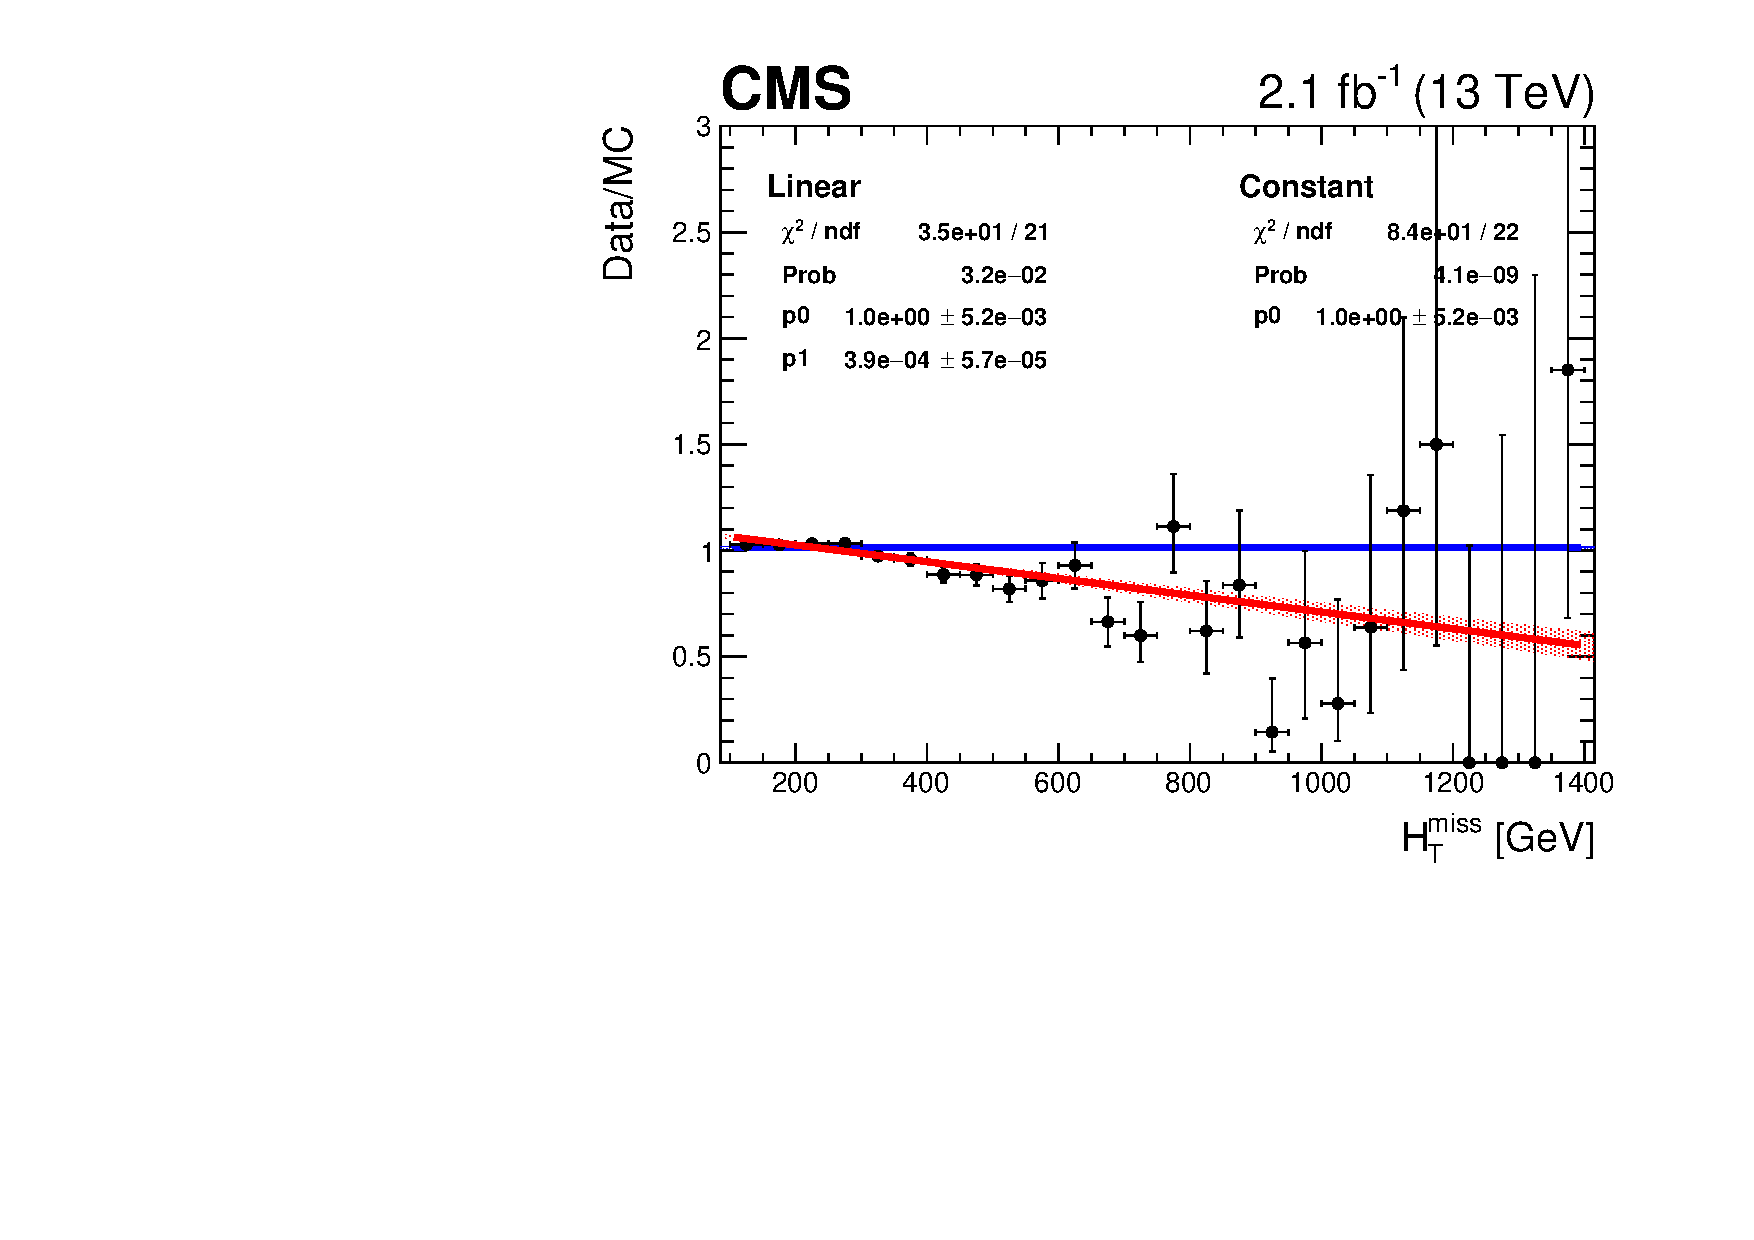
\includegraphics[width=0.5\textwidth]{figures/template2016Data/shapeOutputNewPUInc/scale_ht_variable_mht/SingleMu/Inc_Inc/finalFits/mht_Inc_Inc_ht_Inc_SingleMu_Graph.pdf}
  }~~
  \subfigure[\gj]{
    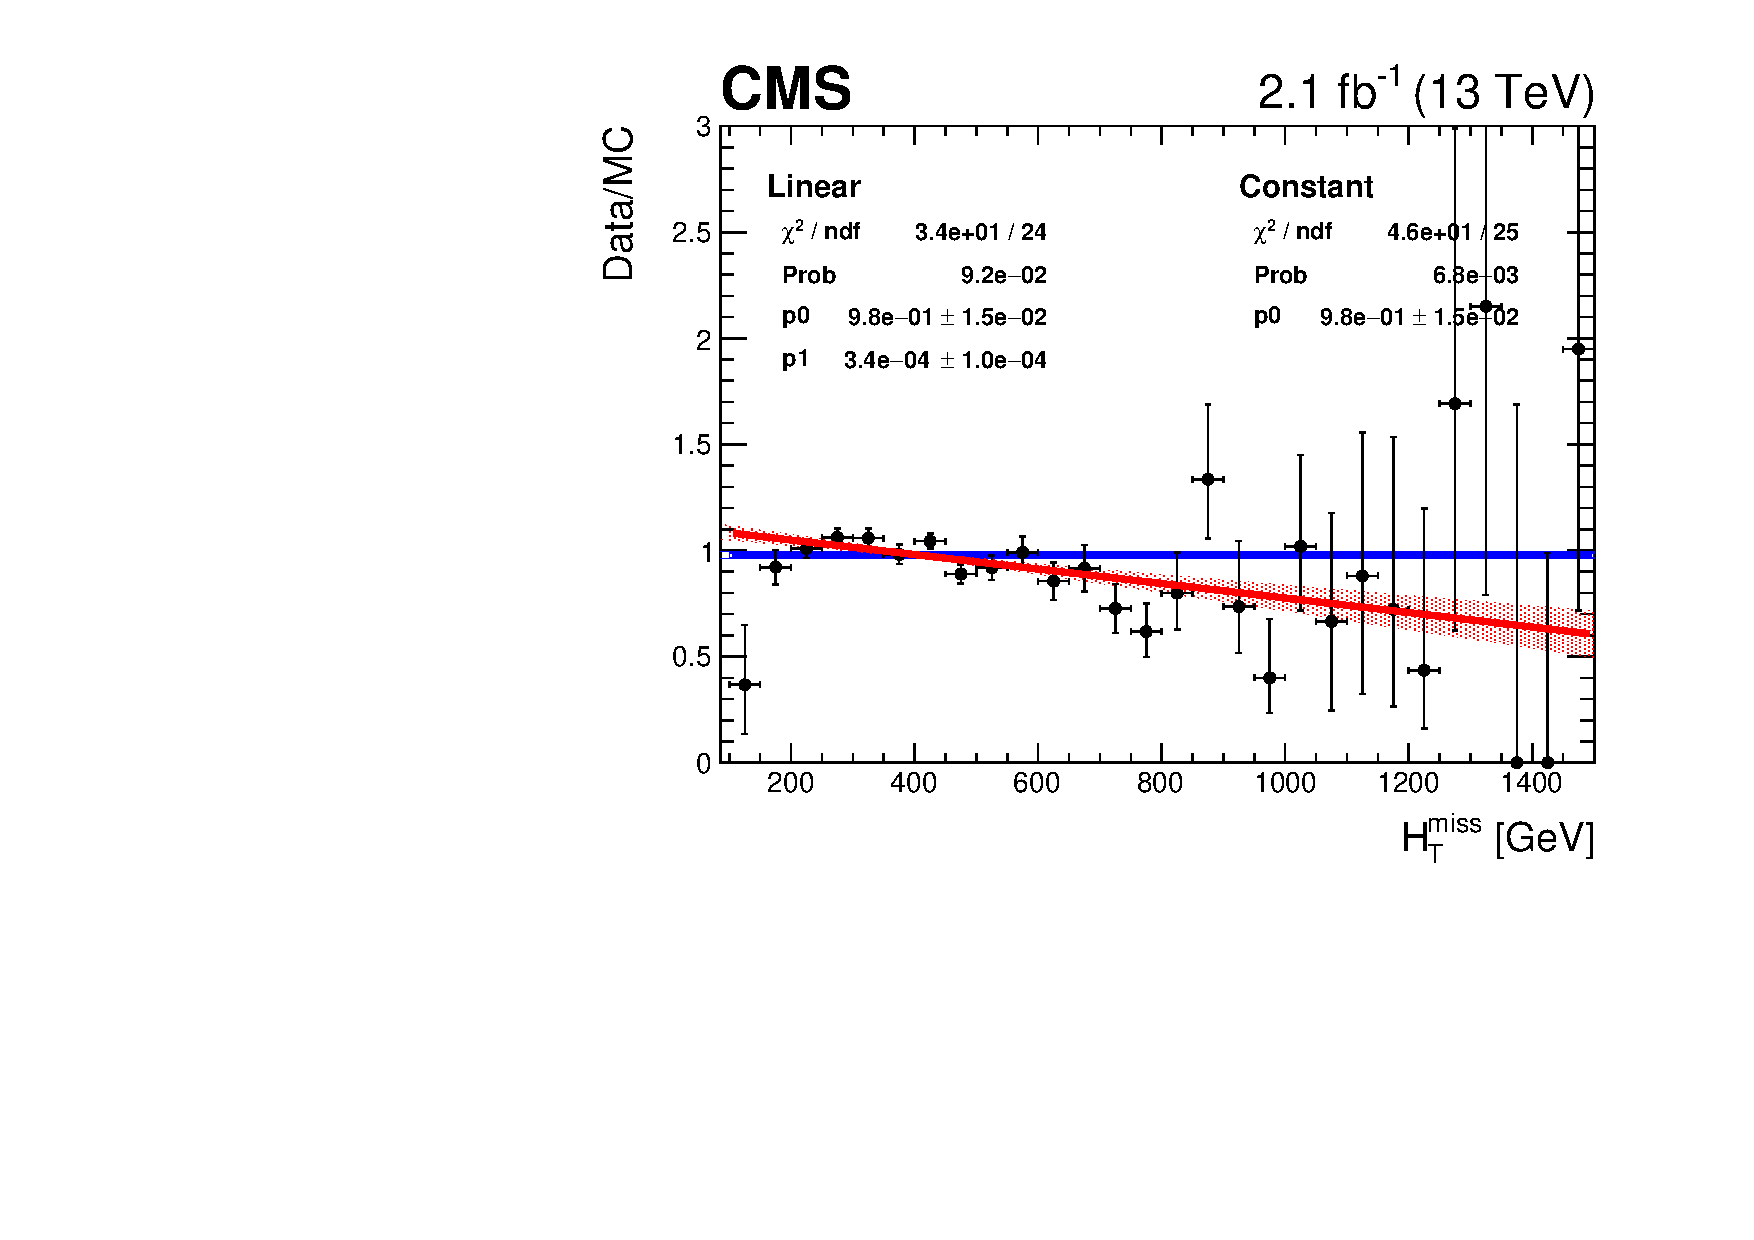
\includegraphics[width=0.5\textwidth]{figures/template2016Data/shapeOutputNewPUInc/scale_ht_variable_mht/SinglePhoton/Inc_Inc/finalFits/mht_Inc_Inc_ht_Inc_SinglePhoton_Graph.pdf}
  }\\
  \subfigure[\mmj]{
    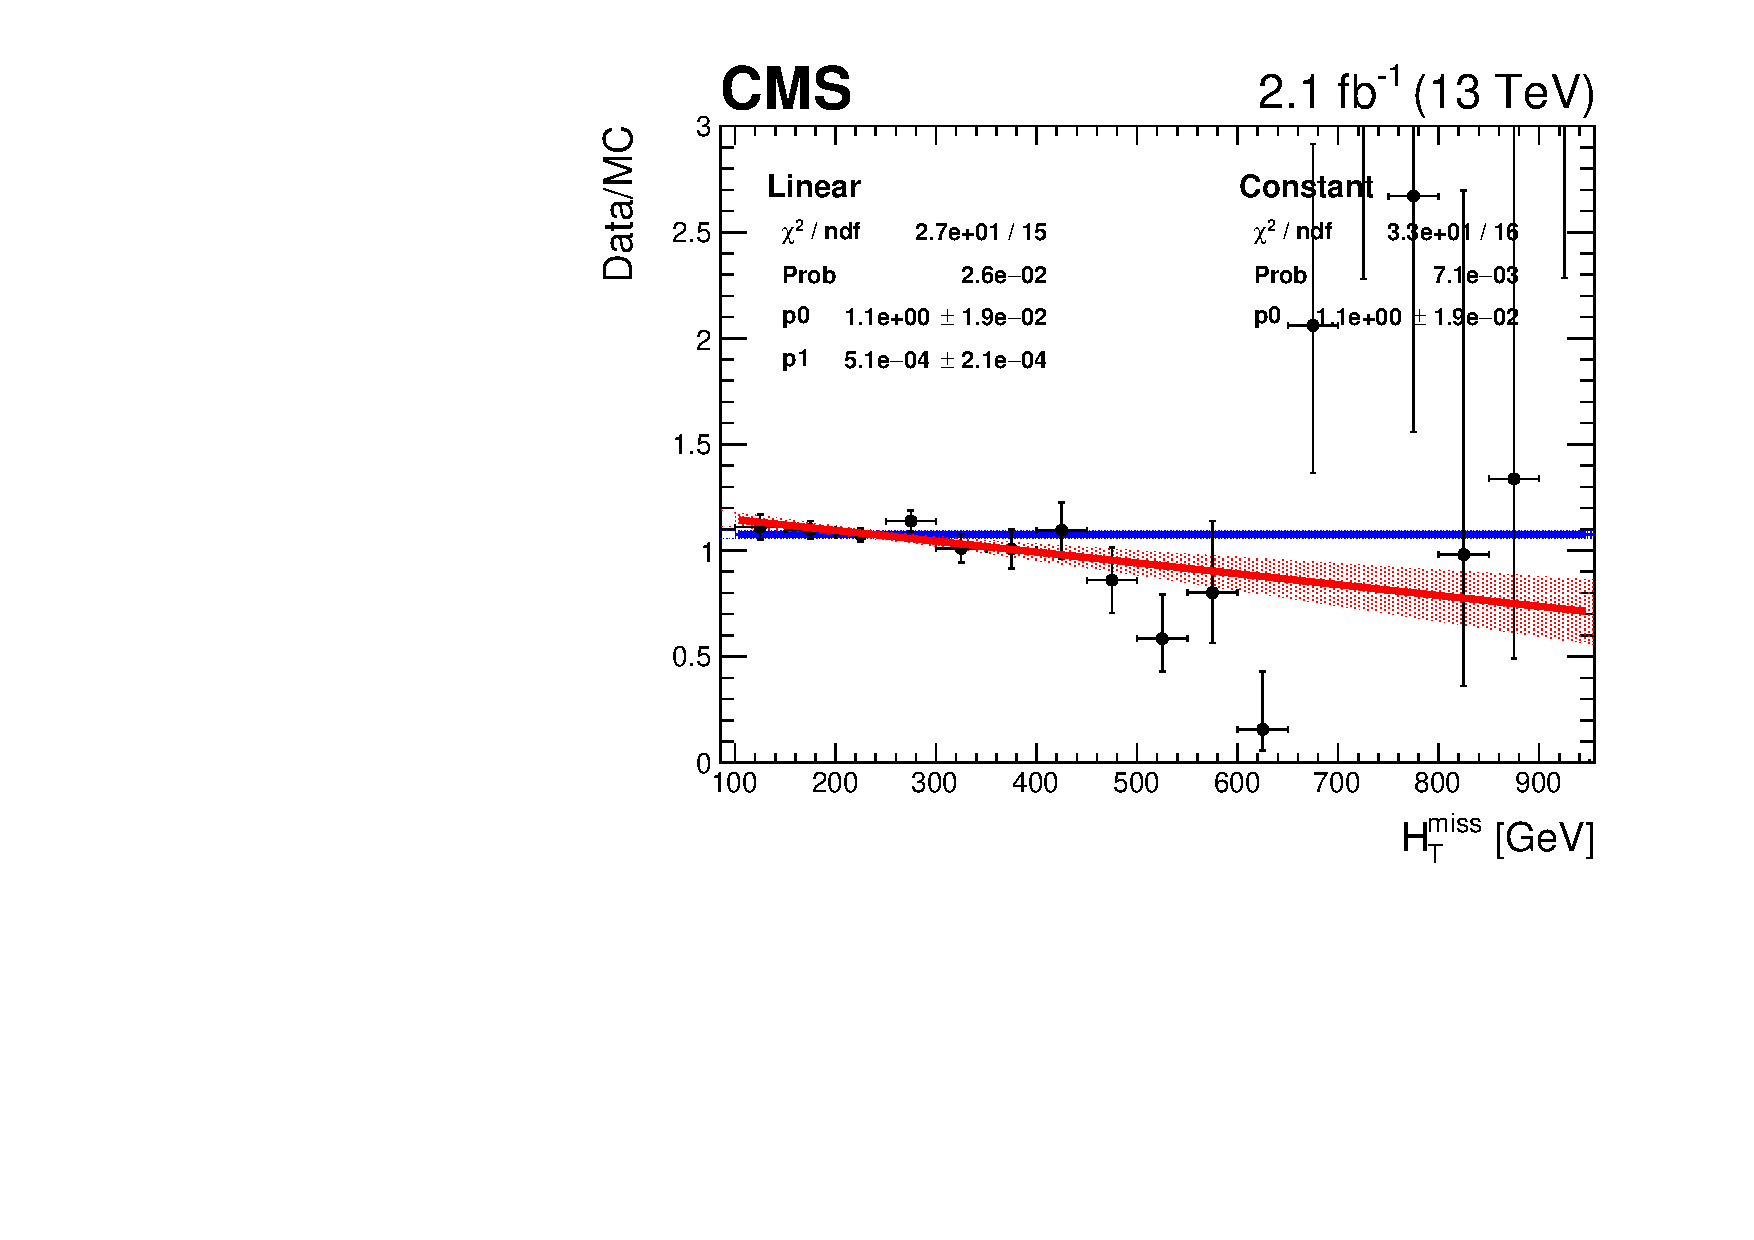
\includegraphics[width=0.5\textwidth]{figures/template2016Data/shapeOutputNewPUInc/scale_ht_variable_mht/DoubleMu/Inc_Inc/finalFits/mht_Inc_Inc_ht_Inc_DoubleMu_Graph.pdf}
  }\\
  \caption{\label{fig:linearMotiv} 
  The data/MC distribution against \mht for an inclusive selection on category and \scalht
  showing the results of a linear fit. A large bias is observed as well as a low pValue for the constant fits. 
 }
\end{figure}

By anchoring the scale using binning in the \scalht dimension the remaining
bias should be negligible. In Fig.~\ref{fig:linearFitExamples} 
example fits of an orthogonal linear function to the data/MC ratio 
are shown for the three control regions. Comparing to the inclusive distribution 
the linear component can be seen to be compatible with the null hypothesis, 
i.e. no bias. In order to formalise this assertion 
the pull of the linear component from zero is calculated.
This pull distribution is shown for each of the three control regions in
in Fig.~\ref{fig:pulls} and can be seen in each case to have mean and sigma
consistent with zero and one respectively. This confirms that the linear component 
is compatible with zero ($p_1 = 0$), i.e. no significant bias is observed, 
and the uncertainty on the parameter is correctly estimated by the fit.
Fig.~\ref{fig:frenchFlagPulls} shows the distribution of the pulls 
in category and \scalht bins. Those anchored by \scalht are consistent
with zero (including inclusive jet categories) while the fits inclusive in \scalht
show very large pulls. This shows, as expected, the \scalht anchoring
is critical for removing bias in the \mht dimension. The linear fits to the
data/MC ratio additionally show a p-value following 
a uniform distribution between 0 and 1 as shown in Fig.~\ref{fig:pValues}.

%Finally, an additional validation 
%can be seen from the p-value distribution of the constant fits
% -- should add p value of constant fit but currently not flat due to
% non guassian behaviour.

\begin{figure}[h!]
  \centering
  \subfigure[\gj, 0b, 2j category and \scalht 800-$\inf$\GeV bin]{
    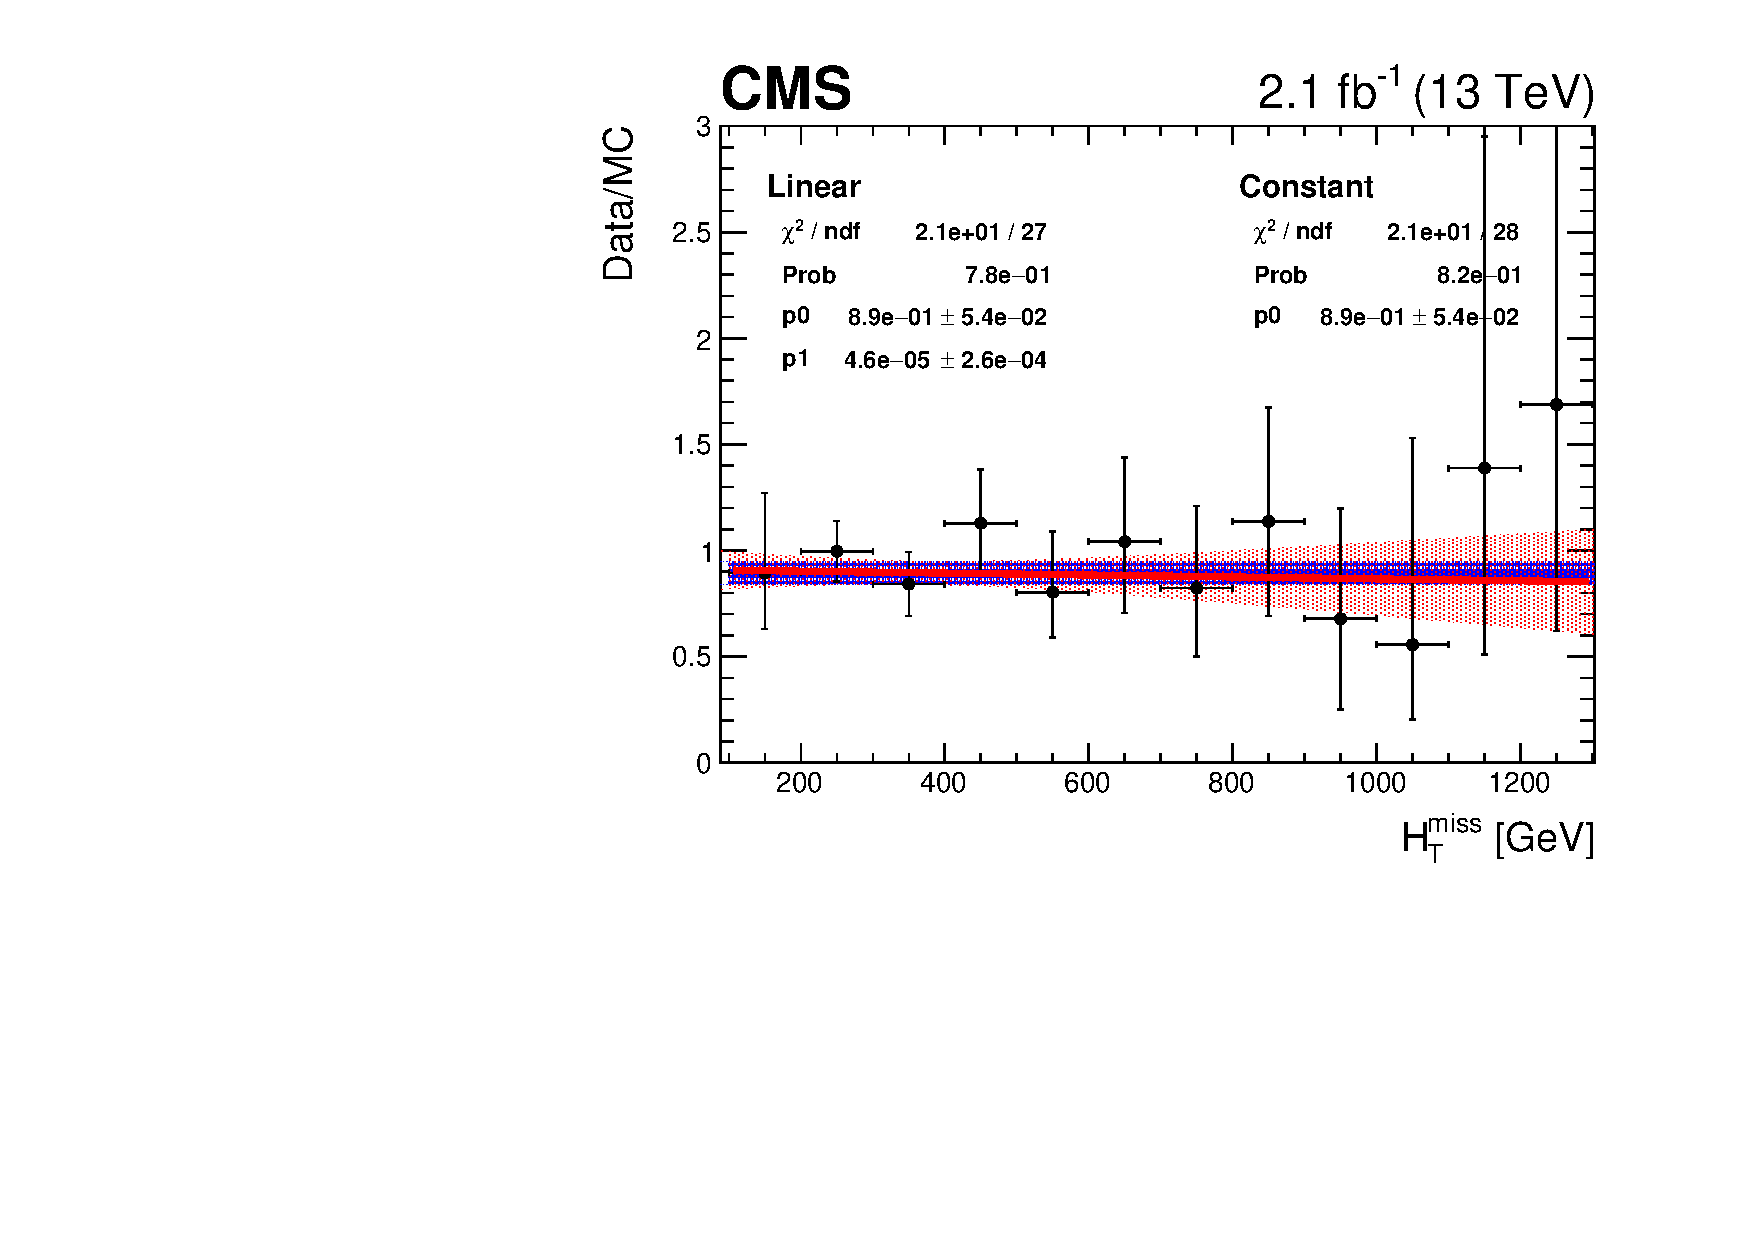
\includegraphics[width=0.5\textwidth]{figures/template2016Data/shapeOutputNewPU/scale_ht_variable_mht/representativeFits/mht_eq0b_eq2j_ht_800_Inf_SinglePhoton_Graph.pdf}
  }~~
  \subfigure[\mj, 1b, 4a category and \scalht 350-400\GeV bin]{
    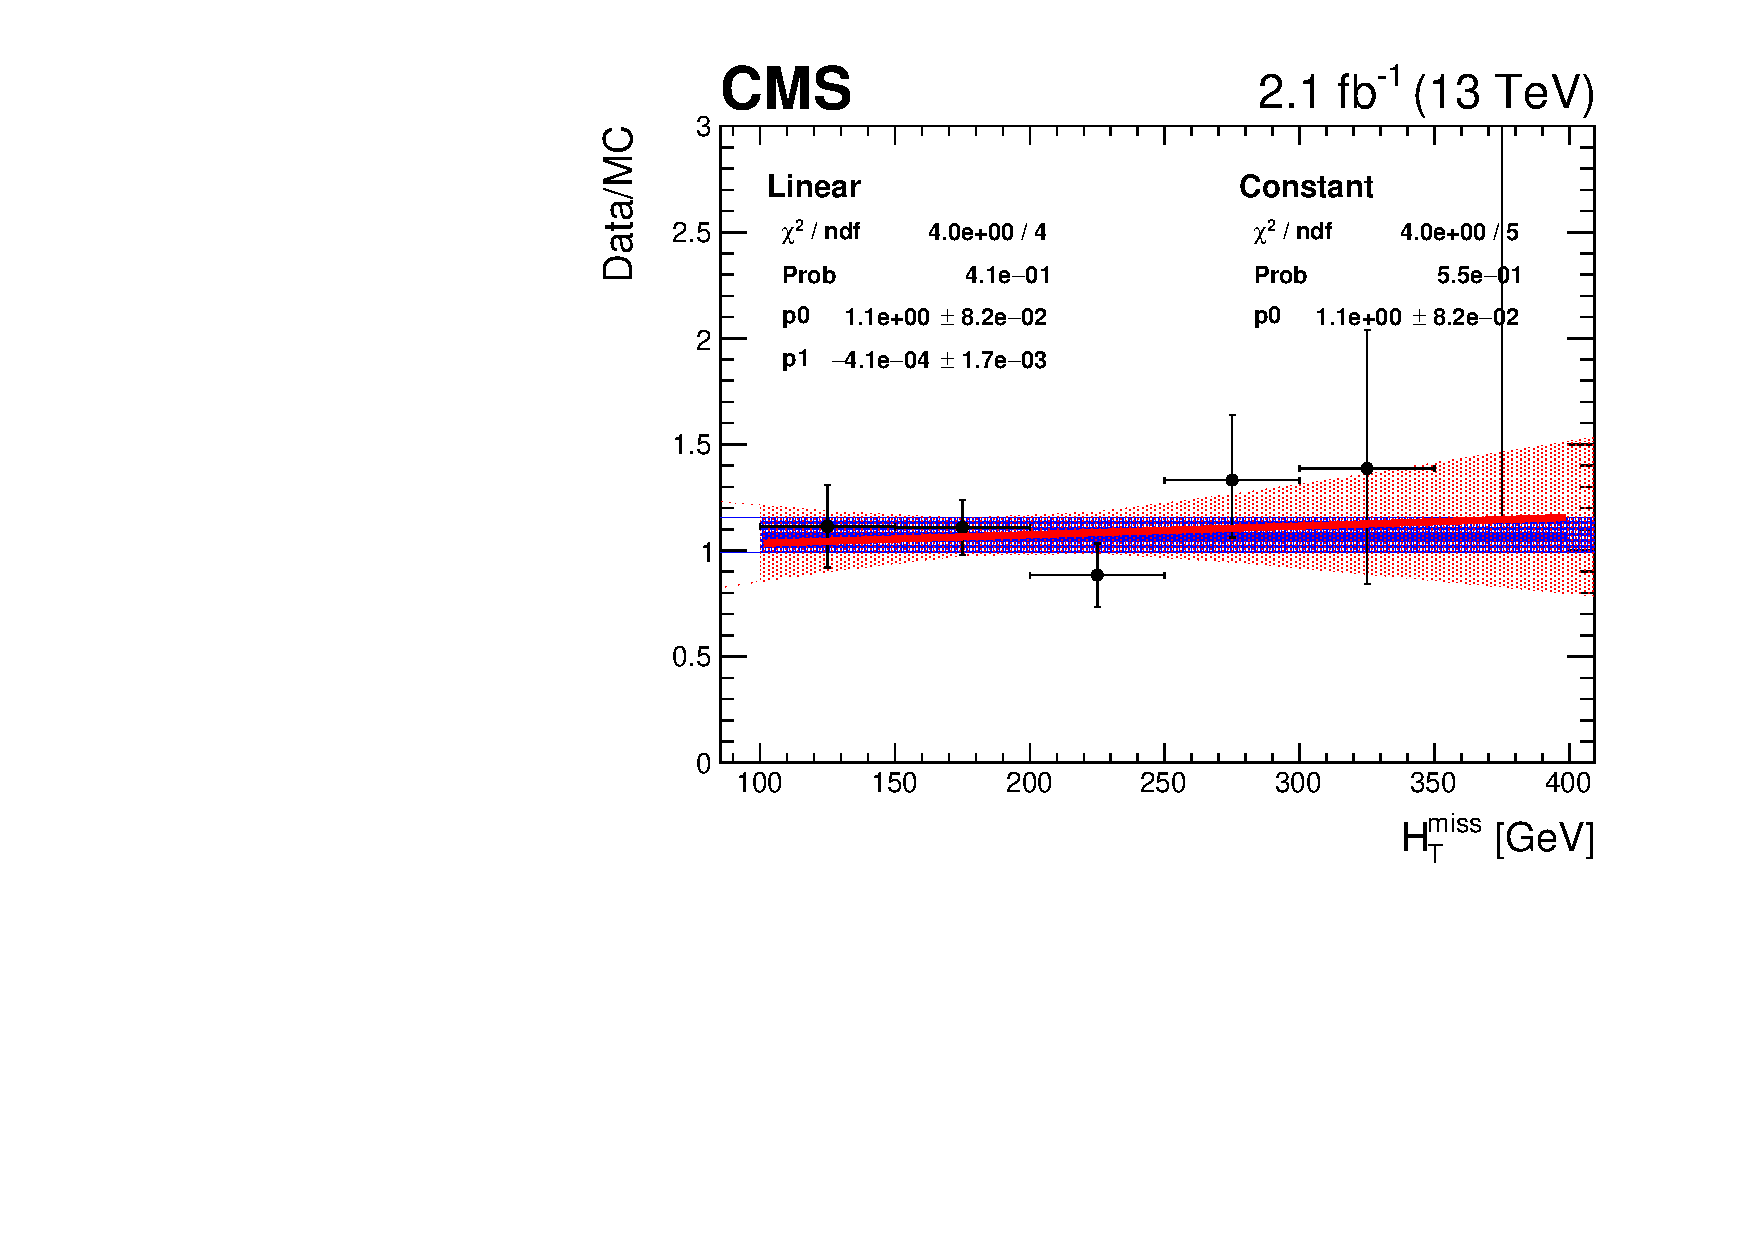
\includegraphics[width=0.5\textwidth]{figures/template2016Data/shapeOutputNewPU/scale_ht_variable_mht/representativeFits/mht_eq1b_eq4a_ht_350_400_SingleMu_Graph.pdf}
  }\\
  \subfigure[\mmj, 0b, 4j category and \scalht 400-500\GeV bin]{
    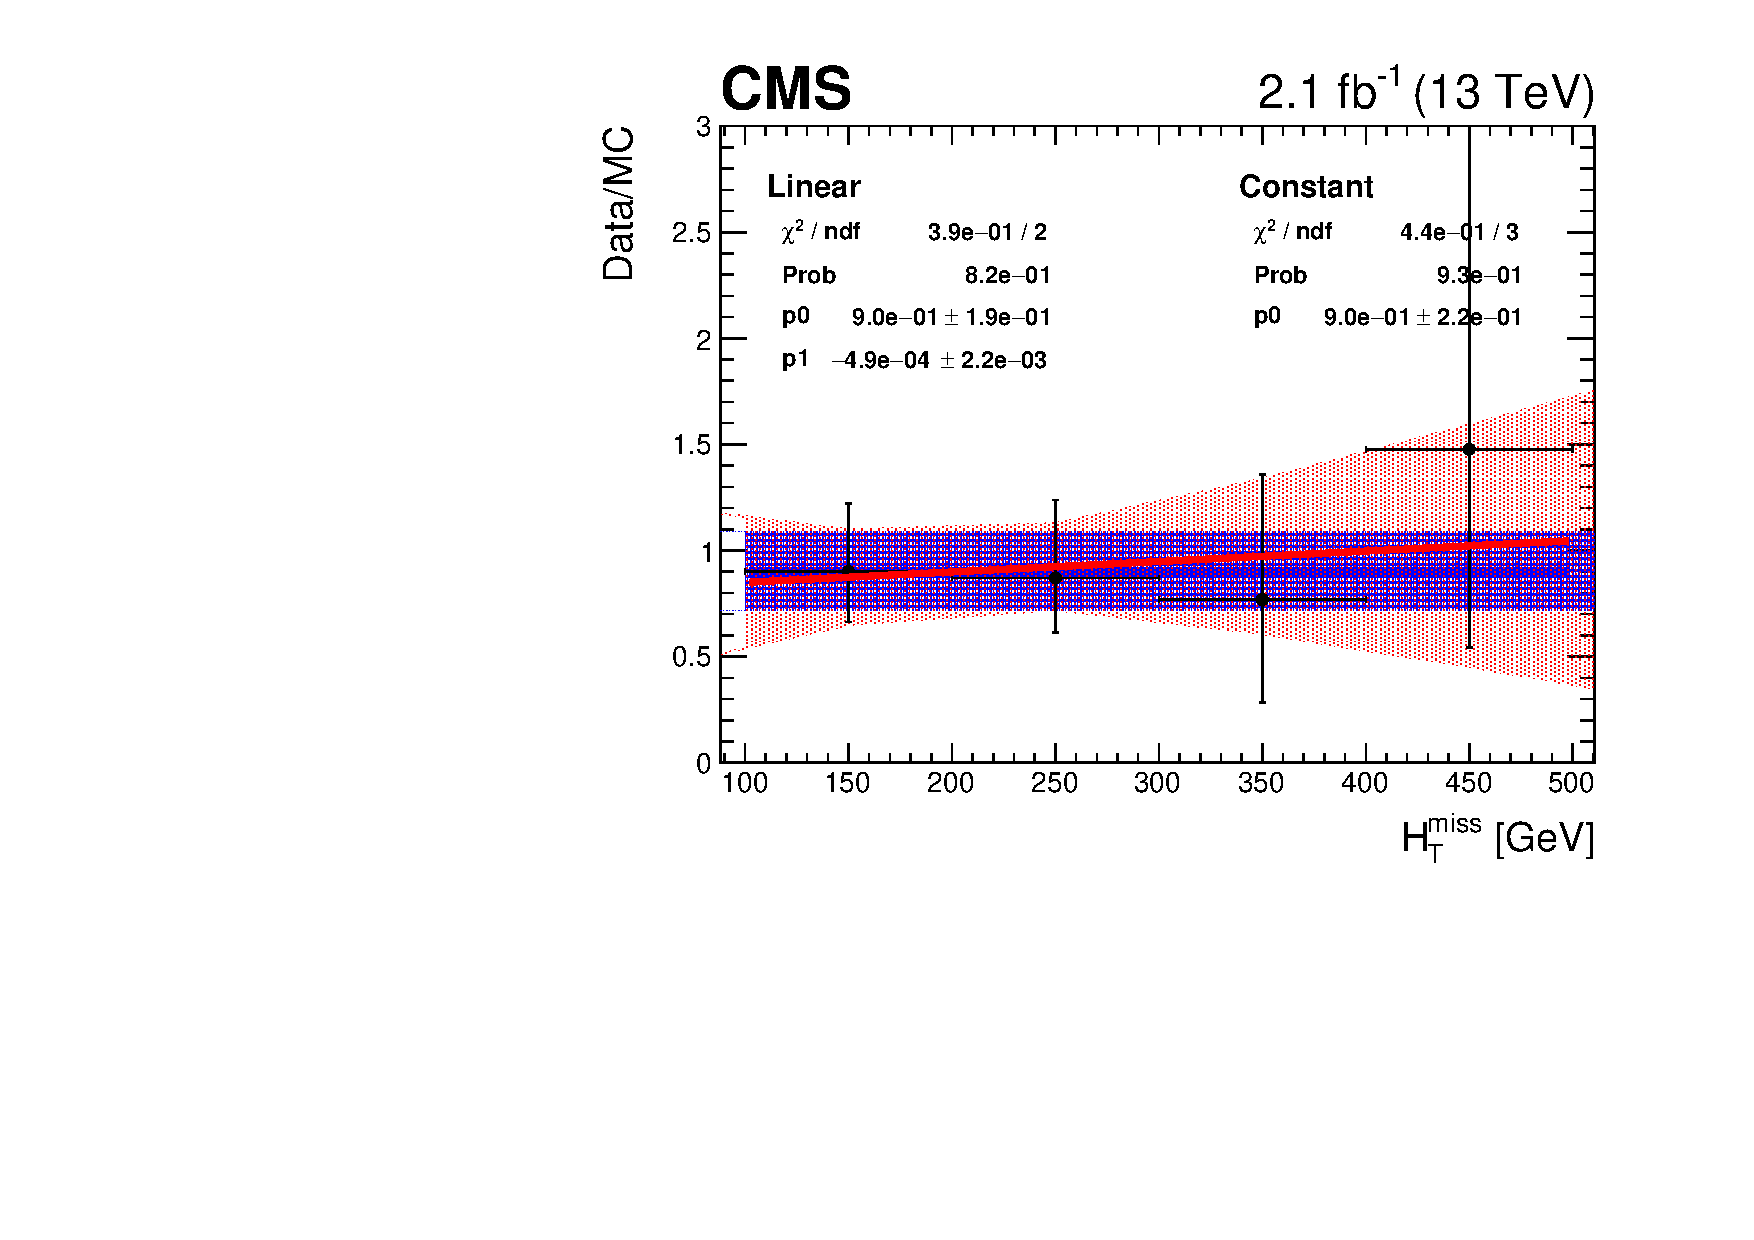
\includegraphics[width=0.5\textwidth]{figures/template2016Data/shapeOutputNewPU/scale_ht_variable_mht/representativeFits/mht_eq0b_eq4j_ht_400_500_DoubleMu_Graph.pdf}
  }~~
  \subfigure[\gj, 1b, 3j category and \scalht 600-800\GeV bin]{
    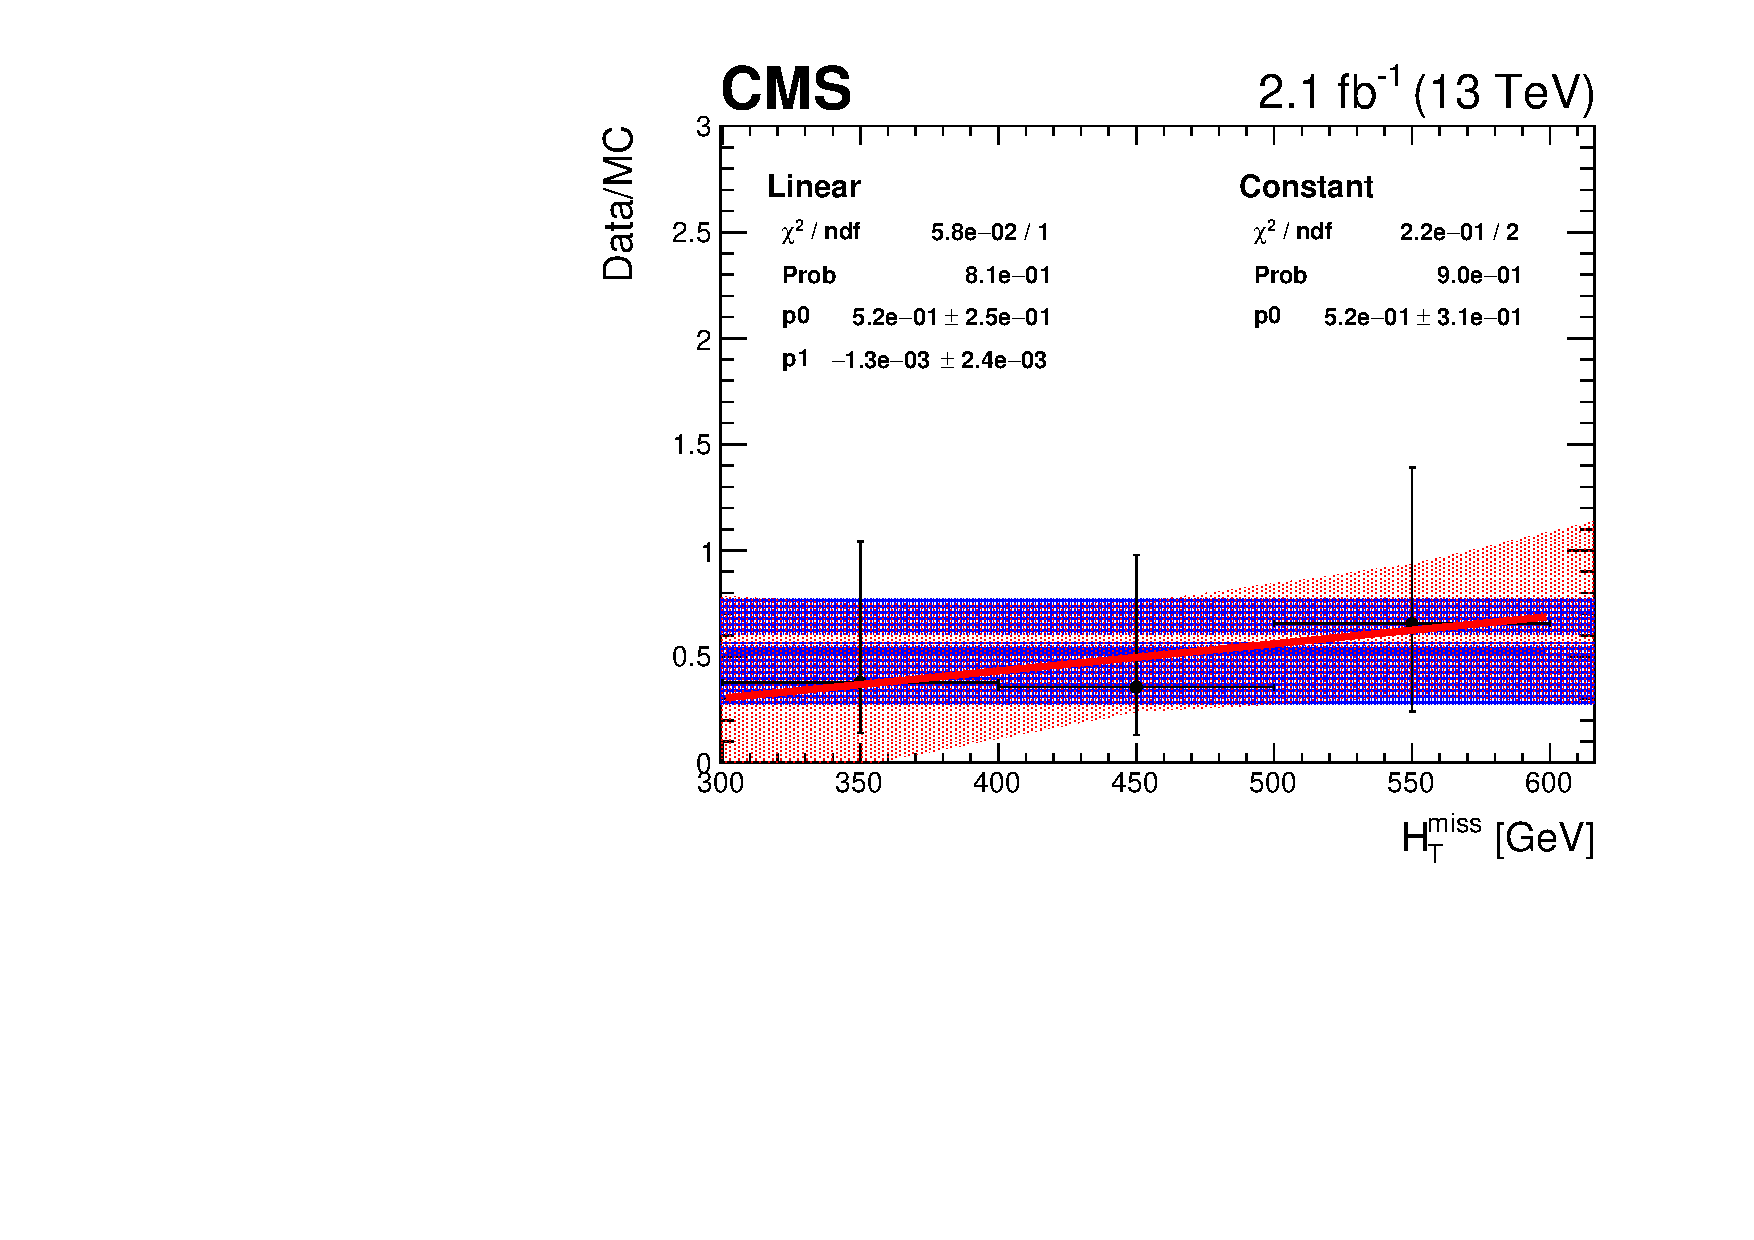
\includegraphics[width=0.5\textwidth]{figures/template2016Data/shapeOutputNewPU/scale_ht_variable_mht/SinglePhoton/eq1b_eq3j/finalFits/mht_eq1b_eq3j_ht_600_800_SinglePhoton_Graph.pdf}
  }\\
  \subfigure[\mj, 2b, 4j category and \scalht 600-800\GeV bin]{
    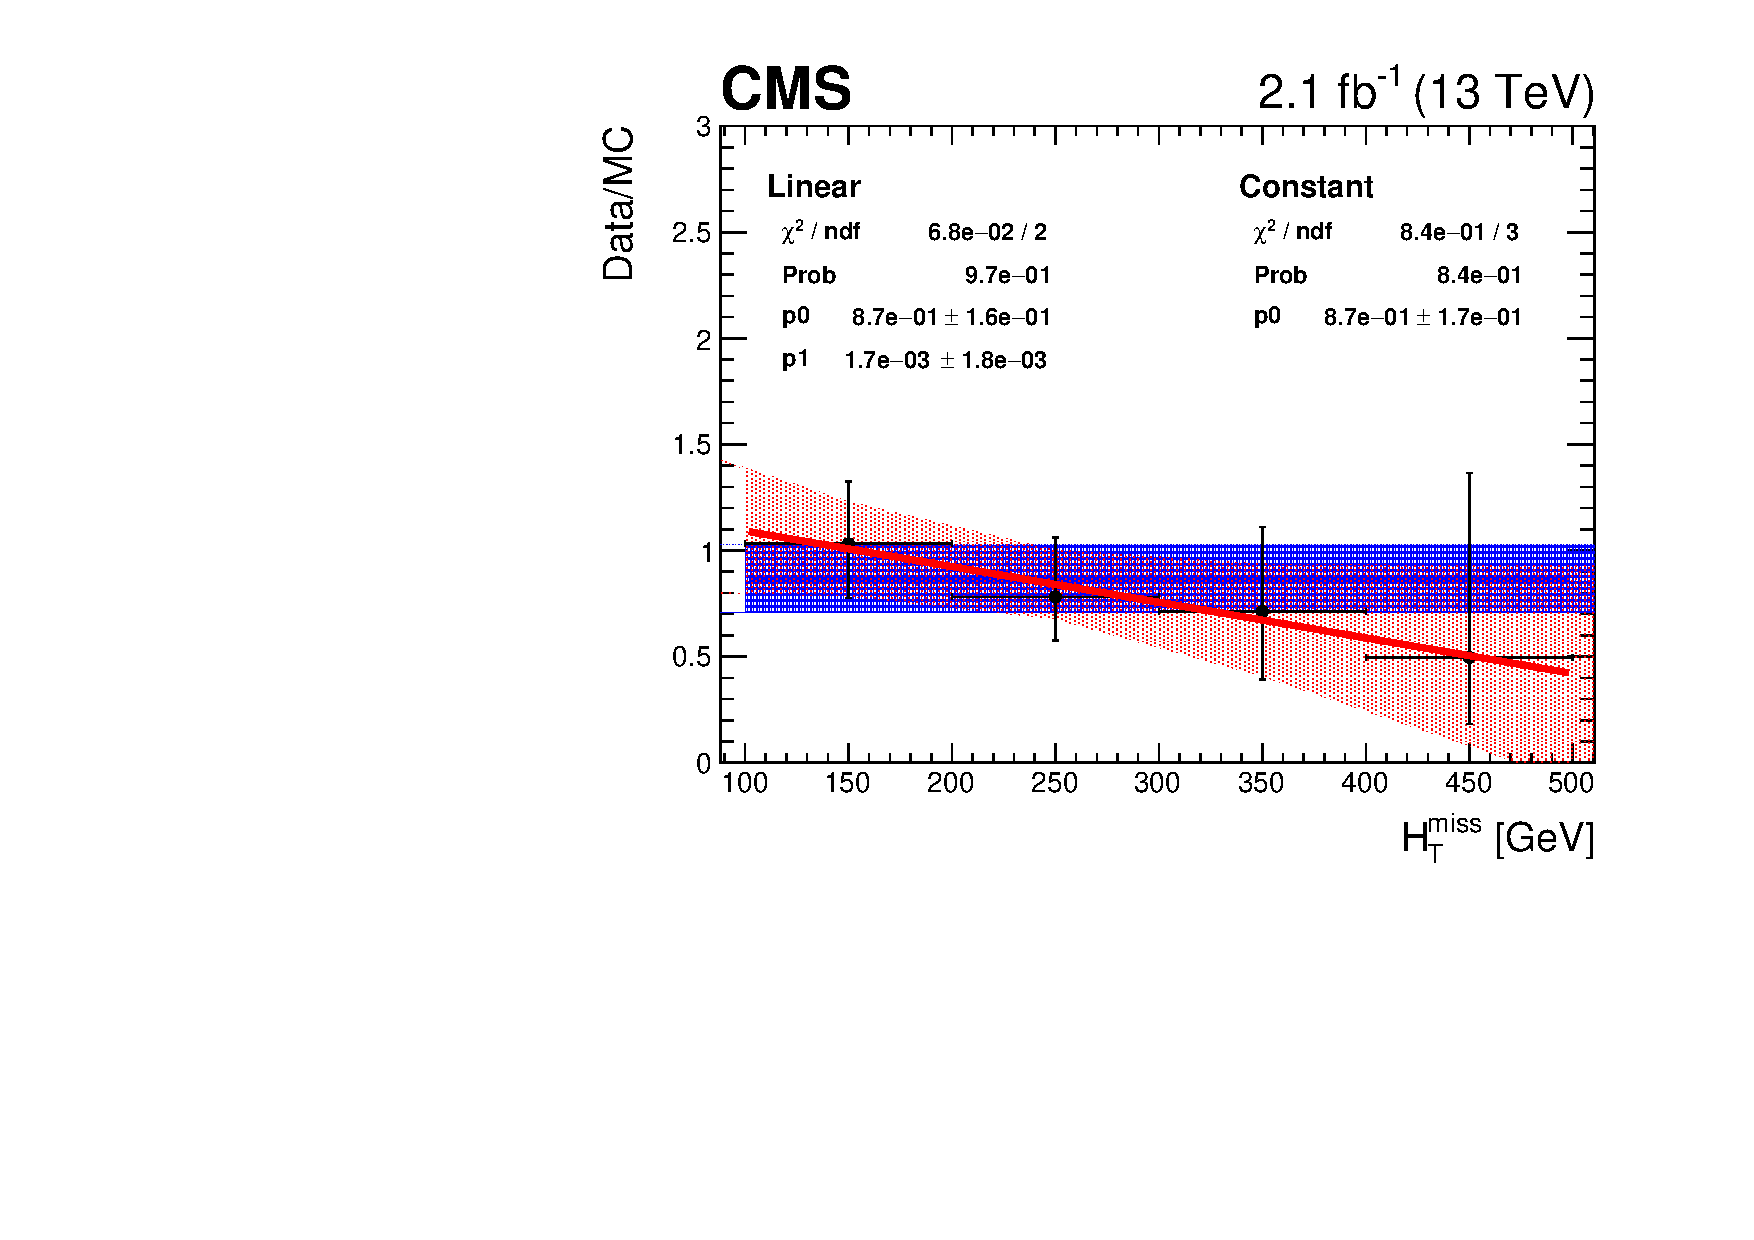
\includegraphics[width=0.5\textwidth]{figures/template2016Data/shapeOutputNewPU/scale_ht_variable_mht/SingleMu/eq2b_eq4j/finalFits/mht_eq2b_eq4j_ht_600_800_SingleMu_Graph.pdf}
  }~~
  \subfigure[\mmj, 0b, 3a category and \scalht 300-350\GeV bin]{
    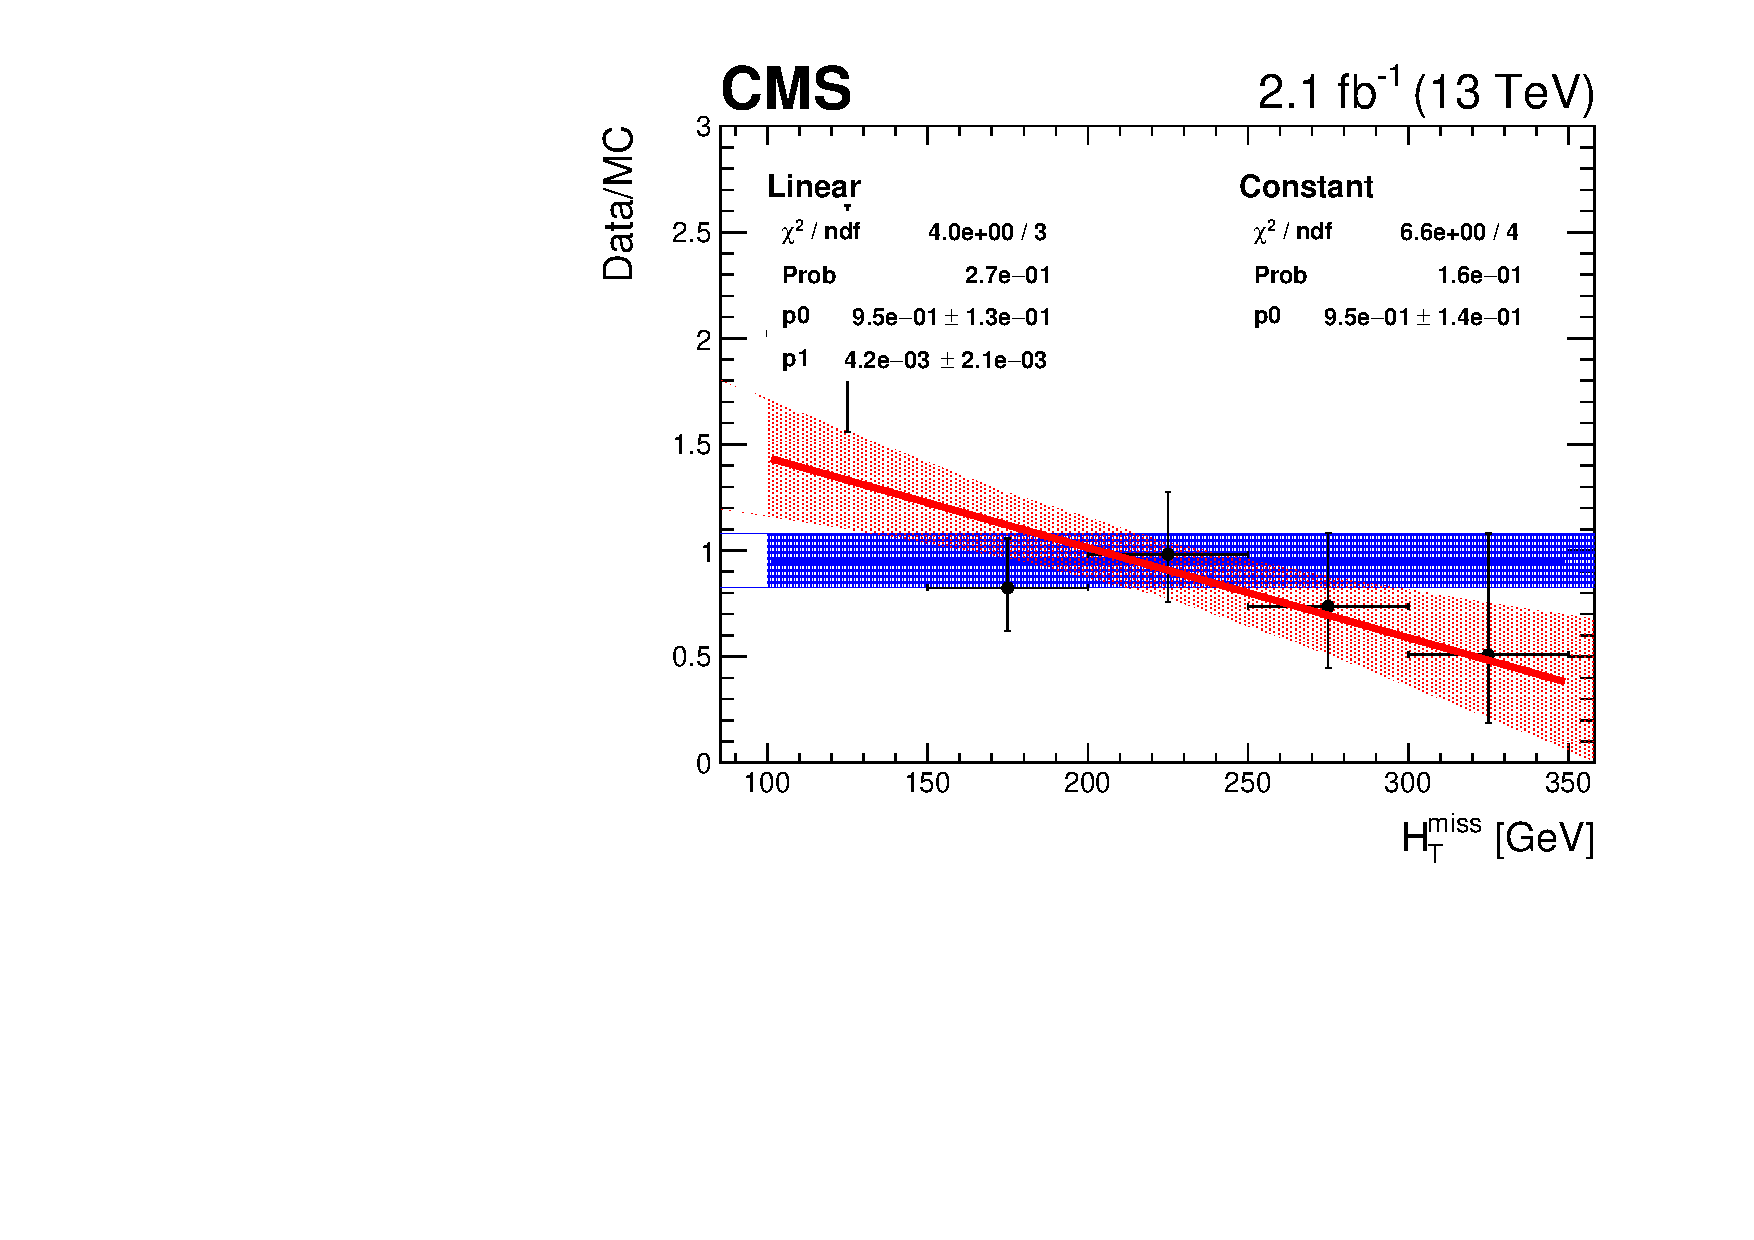
\includegraphics[width=0.5\textwidth]{figures/template2016Data/shapeOutputNewPU/scale_ht_variable_mht/DoubleMu/eq0b_eq3a/finalFits/mht_eq0b_eq3a_ht_300_350_DoubleMu_Graph.pdf}
  }\\
  \caption{\label{fig:linearFitExamples} 
  The data/MC distribution against \mht for example categories and control regions.
  The large bias in the linear component seen in Fig.~\ref{fig:linearMotiv} is mitigated.}
\end{figure}

\begin{figure}[h!]
  \centering
  \subfigure[\mj]{
    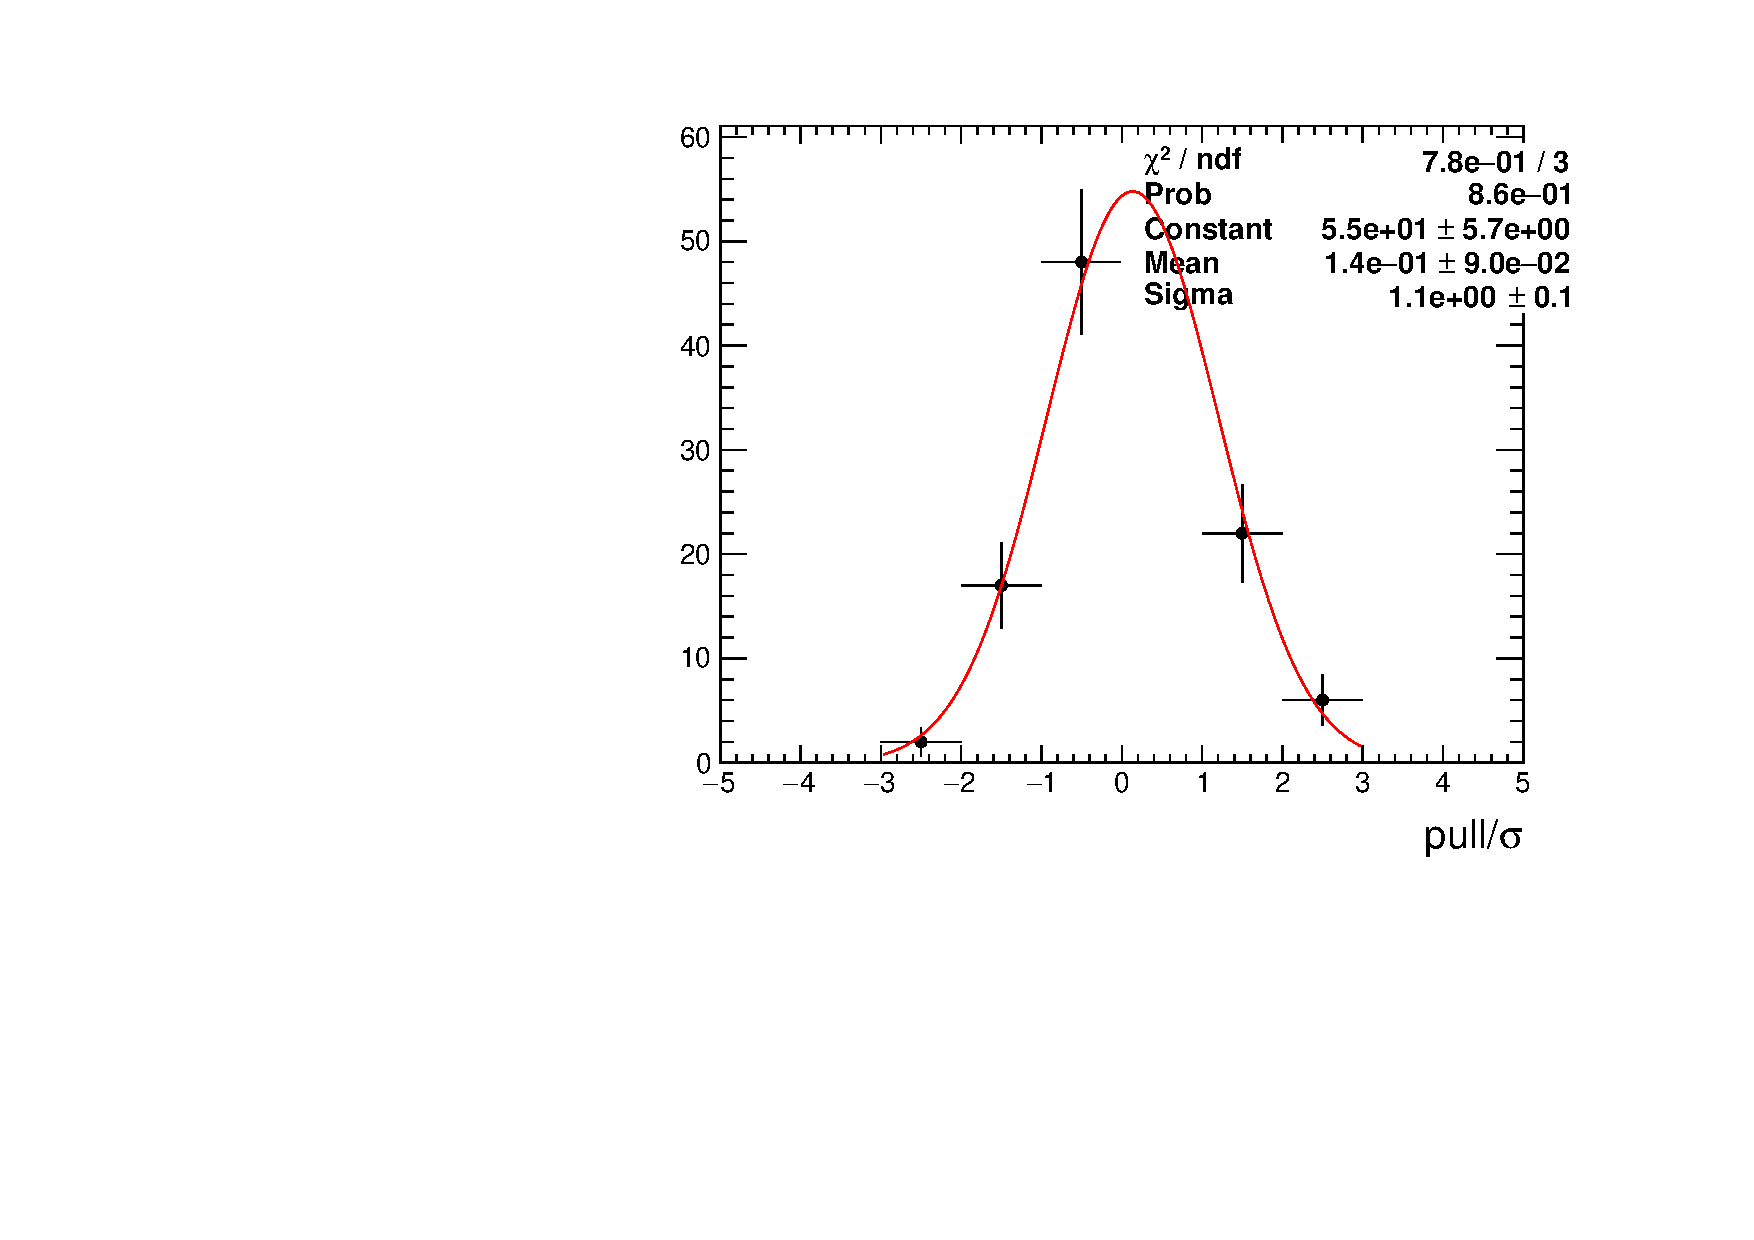
\includegraphics[width=0.5\textwidth]{figures/template2016Data/shapeOutputNewPU/scale_ht_variable_mht/SingleMu/fitOut/Linear2DShiftMean/pull_Linear2DShiftMean_p1_SingleMu.pdf}
  }~~
  \subfigure[\gj]{
    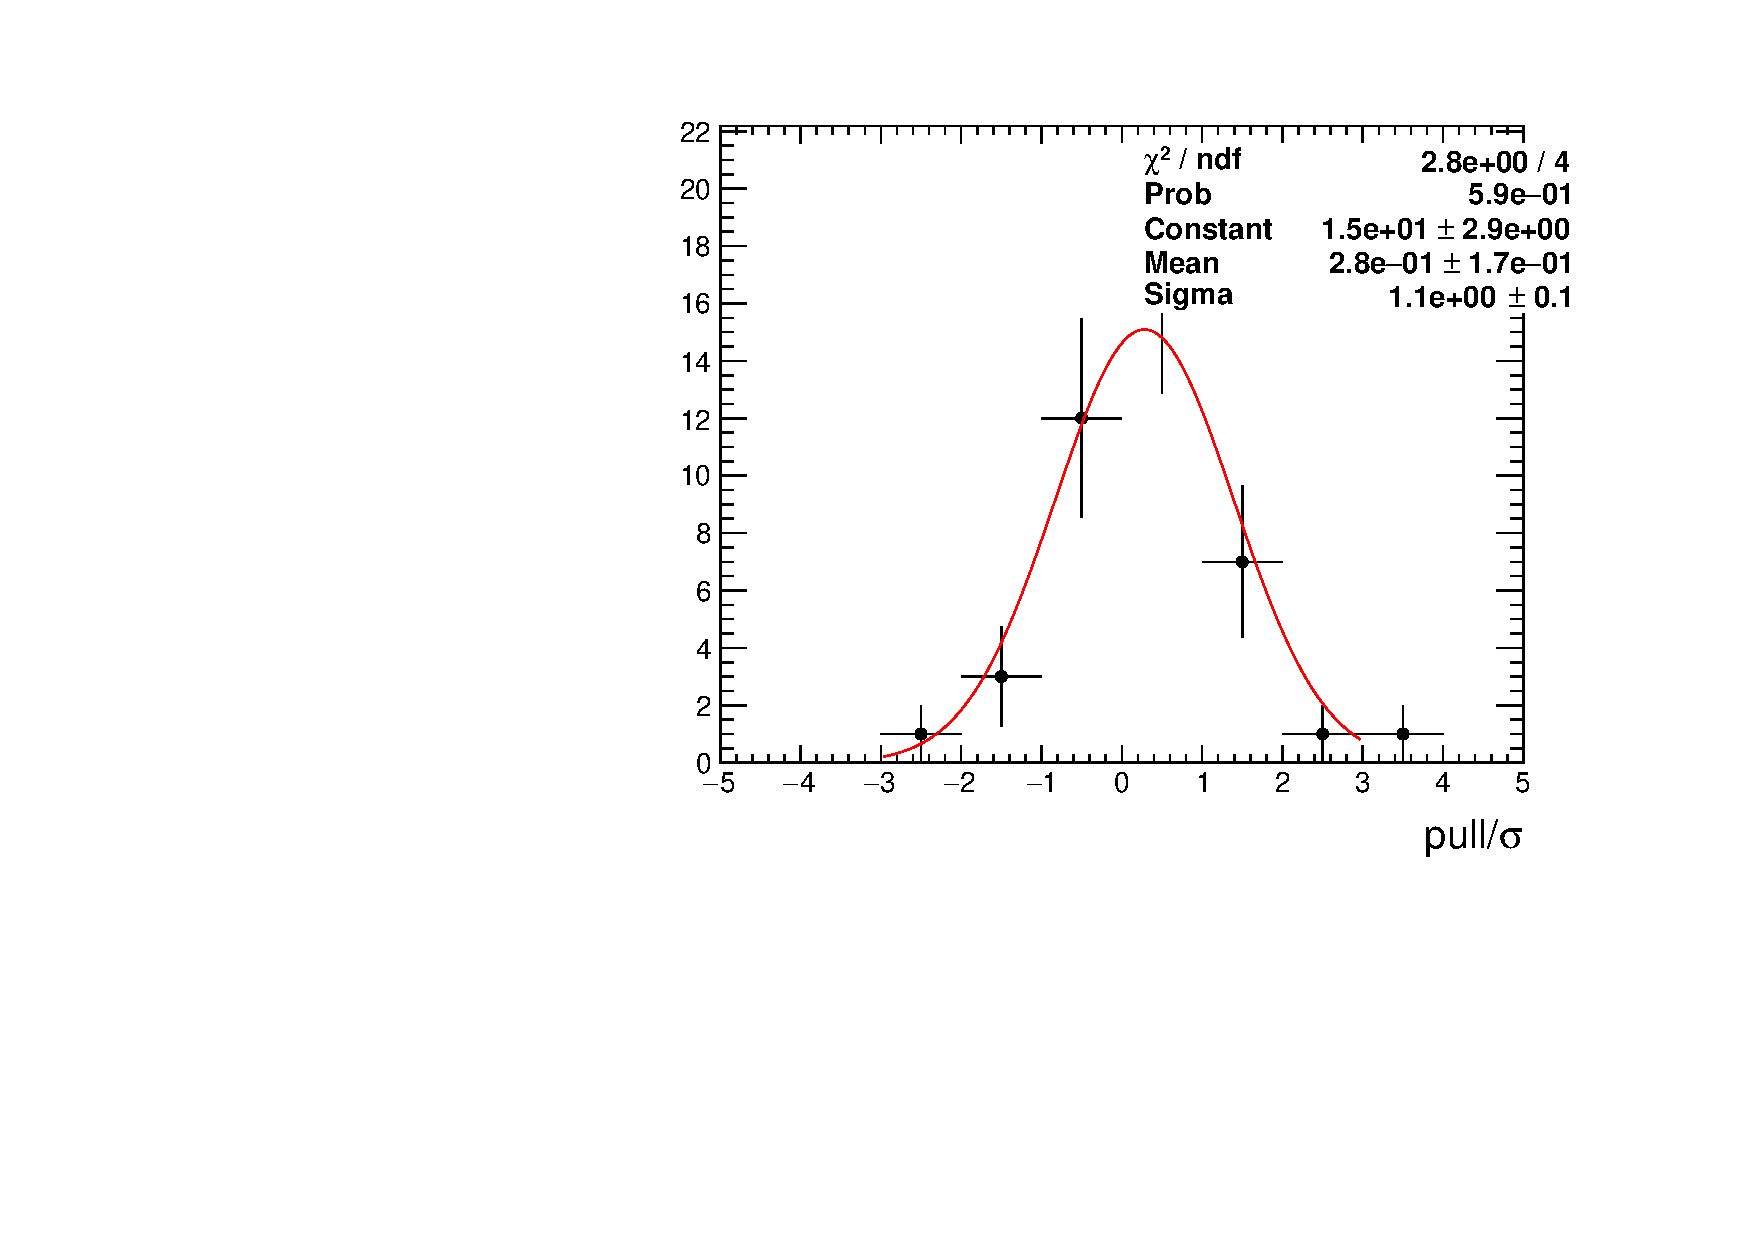
\includegraphics[width=0.5\textwidth]{figures/template2016Data/shapeOutputNewPU/scale_ht_variable_mht/SinglePhoton/fitOut/Linear2DShiftMean/pull_Linear2DShiftMean_p1_SinglePhoton.pdf}
  }\\
  \subfigure[\mmj]{
    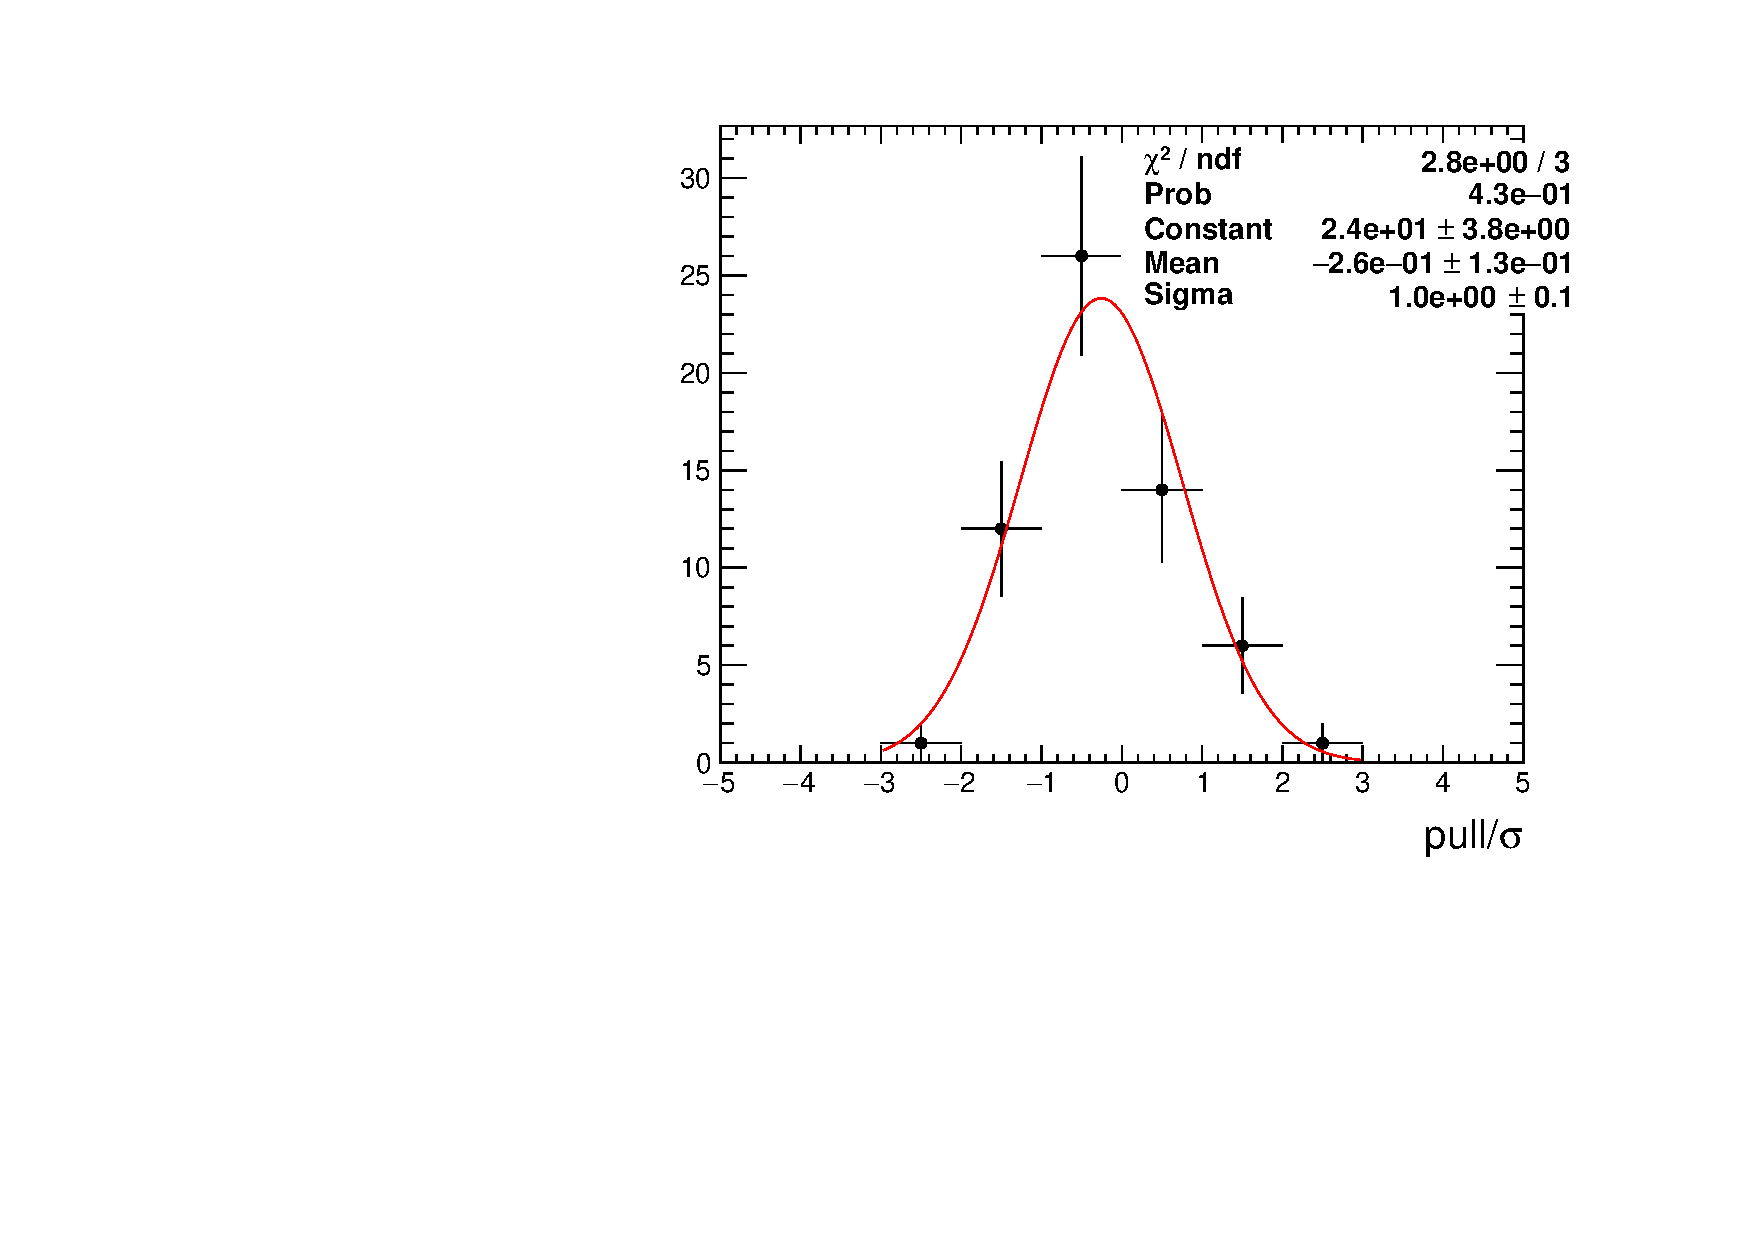
\includegraphics[width=0.5\textwidth]{figures/template2016Data/shapeOutputNewPU/scale_ht_variable_mht/DoubleMu/fitOut/Linear2DShiftMean/pull_Linear2DShiftMean_p1_DoubleMu.pdf}
  }~~
  \\
  \caption{\label{fig:pulls} 
  The pull distribution of the linear parameter from the flat hypothesis showing no significant bias.}
\end{figure}
\begin{figure}[h!]
  \centering
  \subfigure[\mj]{
    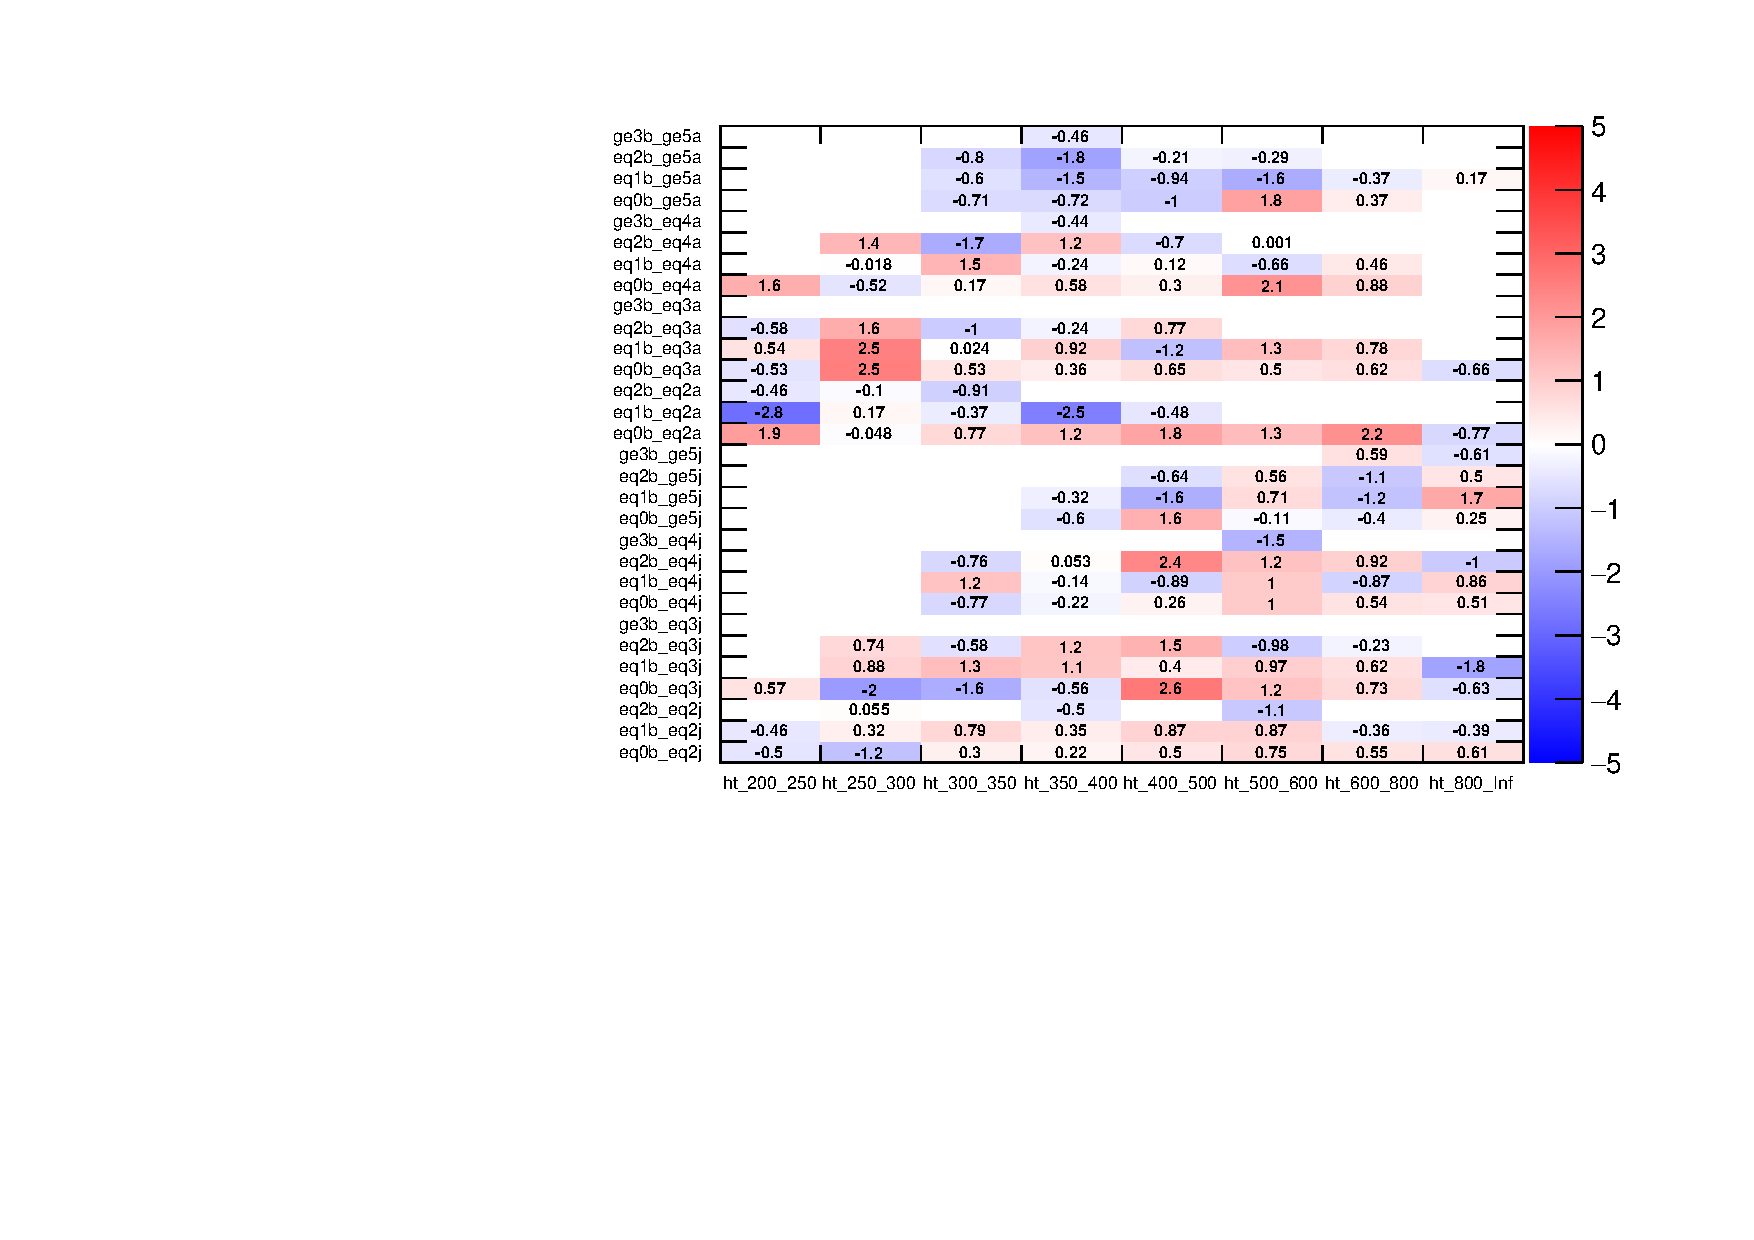
\includegraphics[width=0.5\textwidth]{figures/template2016Data/shapeOutputNewPU/scale_ht_variable_mht/SingleMu/fitOut/Linear2DShiftMean/frenchFlagPull_Linear2DShiftMean_p1_SingleMu.pdf}
  }~~
  \subfigure[\gj]{
    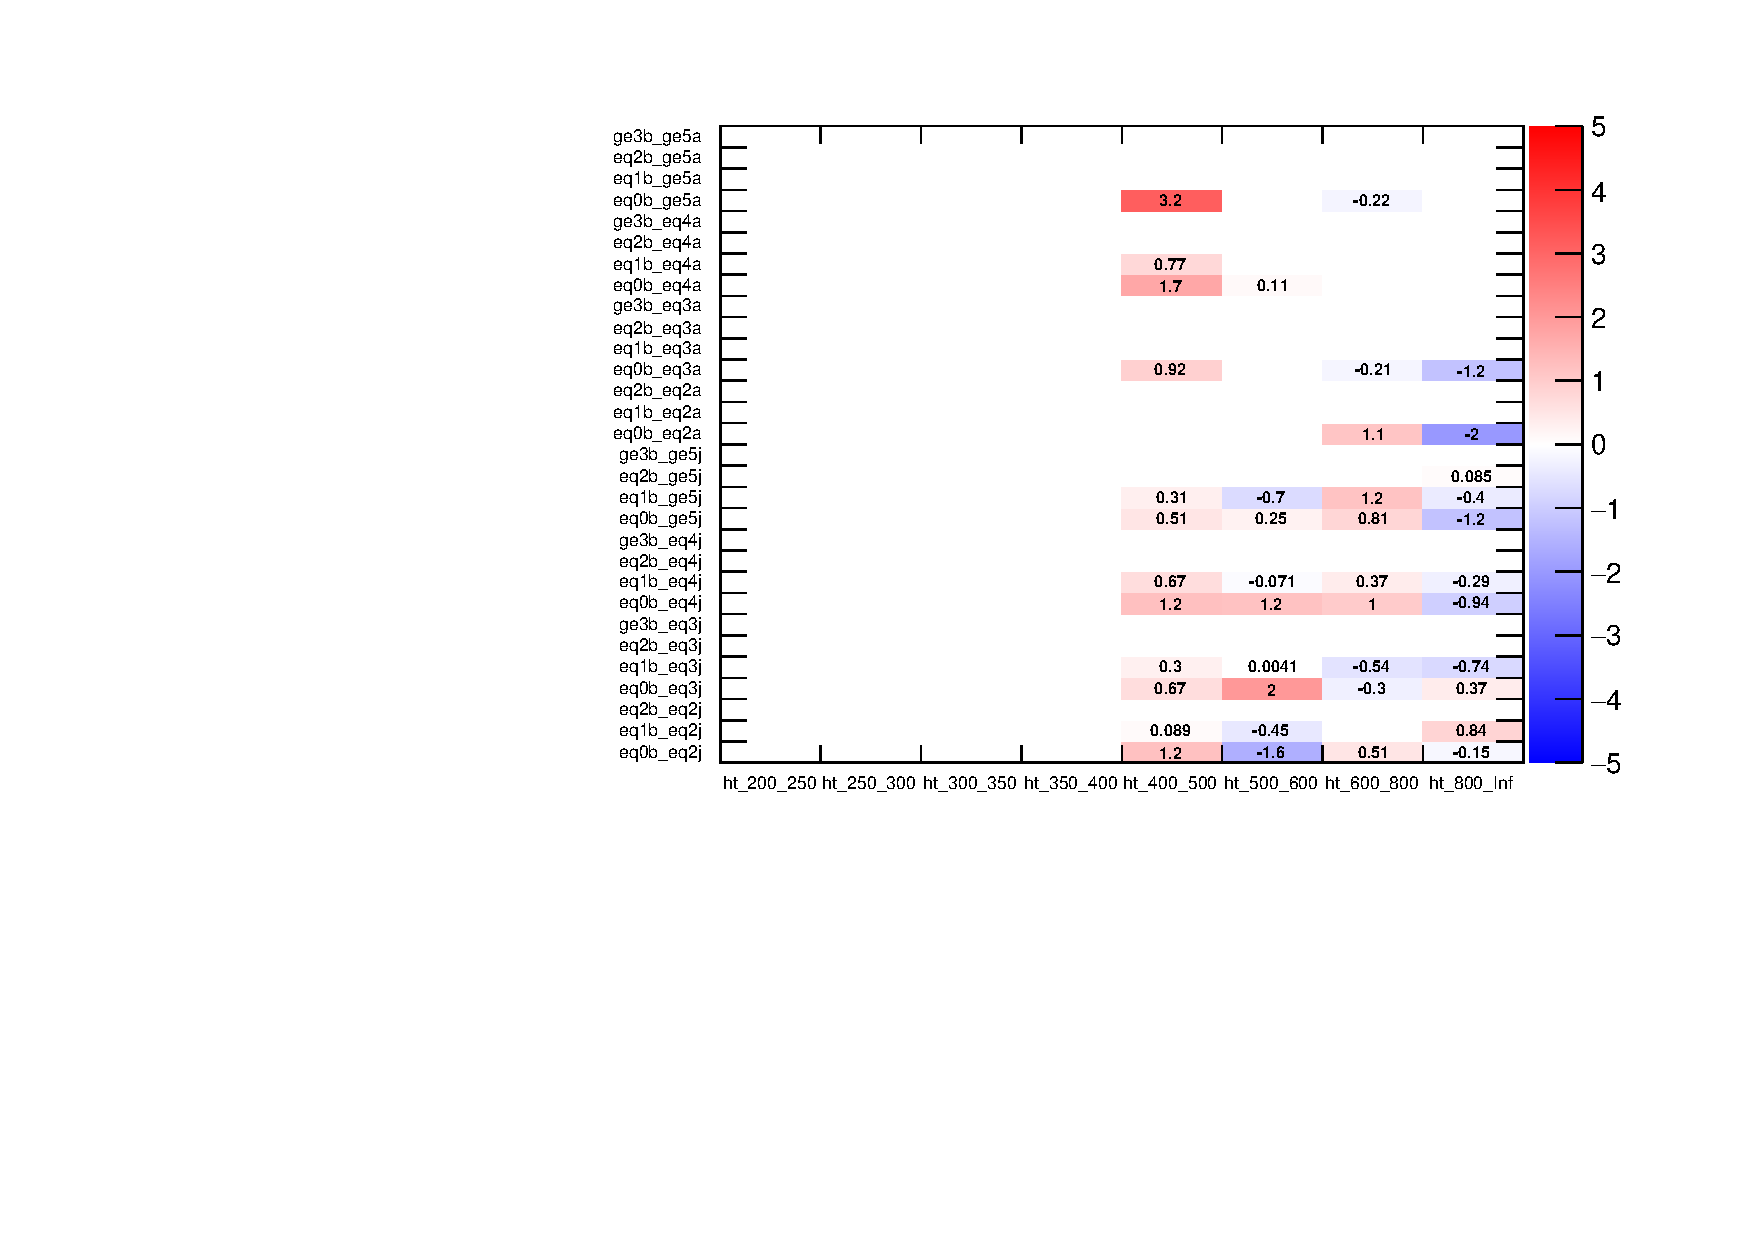
\includegraphics[width=0.5\textwidth]{figures/template2016Data/shapeOutputNewPU/scale_ht_variable_mht/SinglePhoton/fitOut/Linear2DShiftMean/frenchFlagPull_Linear2DShiftMean_p1_SinglePhoton.pdf}
  }\\
  \subfigure[\mmj]{
    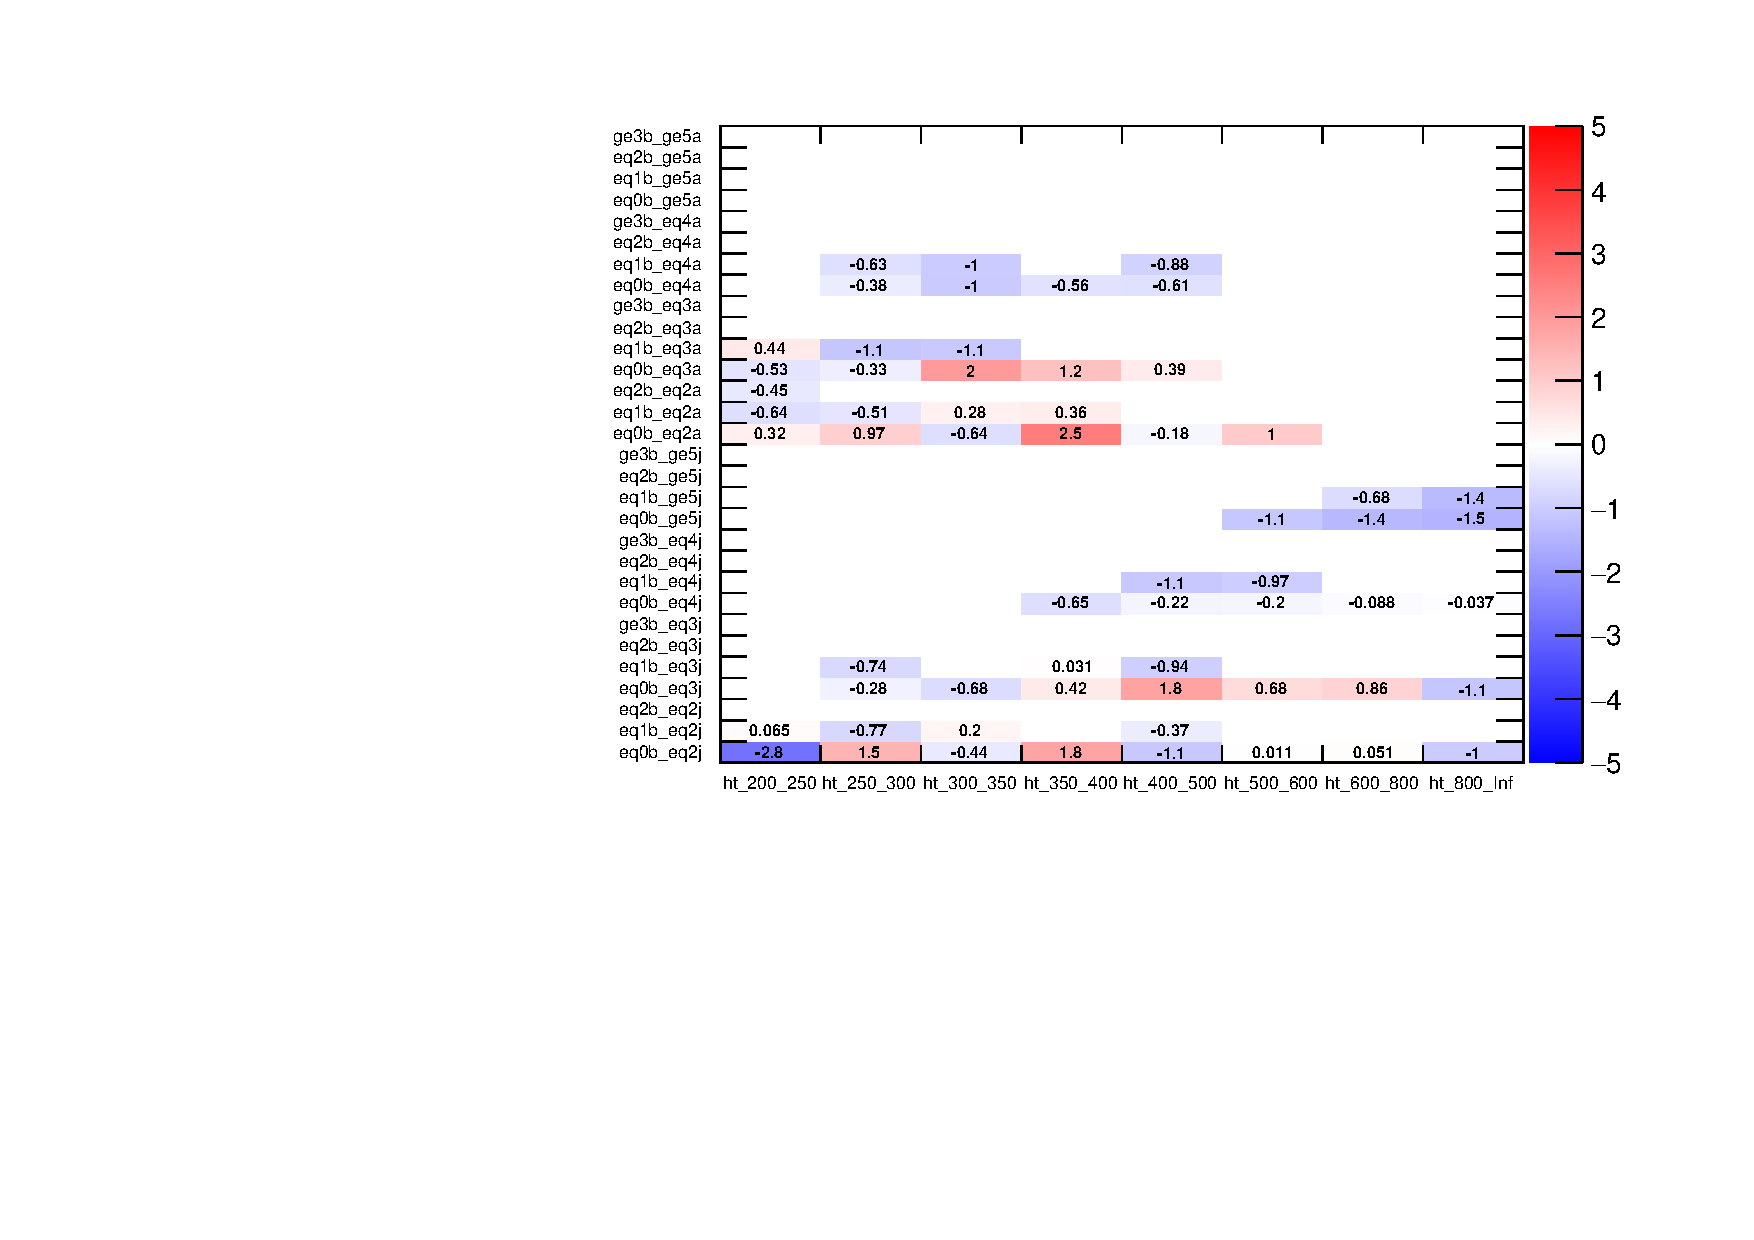
\includegraphics[width=0.5\textwidth]{figures/template2016Data/shapeOutputNewPU/scale_ht_variable_mht/DoubleMu/fitOut/Linear2DShiftMean/frenchFlagPull_Linear2DShiftMean_p1_DoubleMu.pdf}
  }~~
  \\
  \caption{\label{fig:frenchFlagPulls} The pull distribution of the linear parameter from the flat hypothesis across all
  \scalht bins and categories. There are no significant pulls for the \scalht binned
  fits while the \scalht inclusive case shows very large pulls as expected.}
\end{figure}

\begin{figure}[h!]
  \centering
  \subfigure[\mj]{
    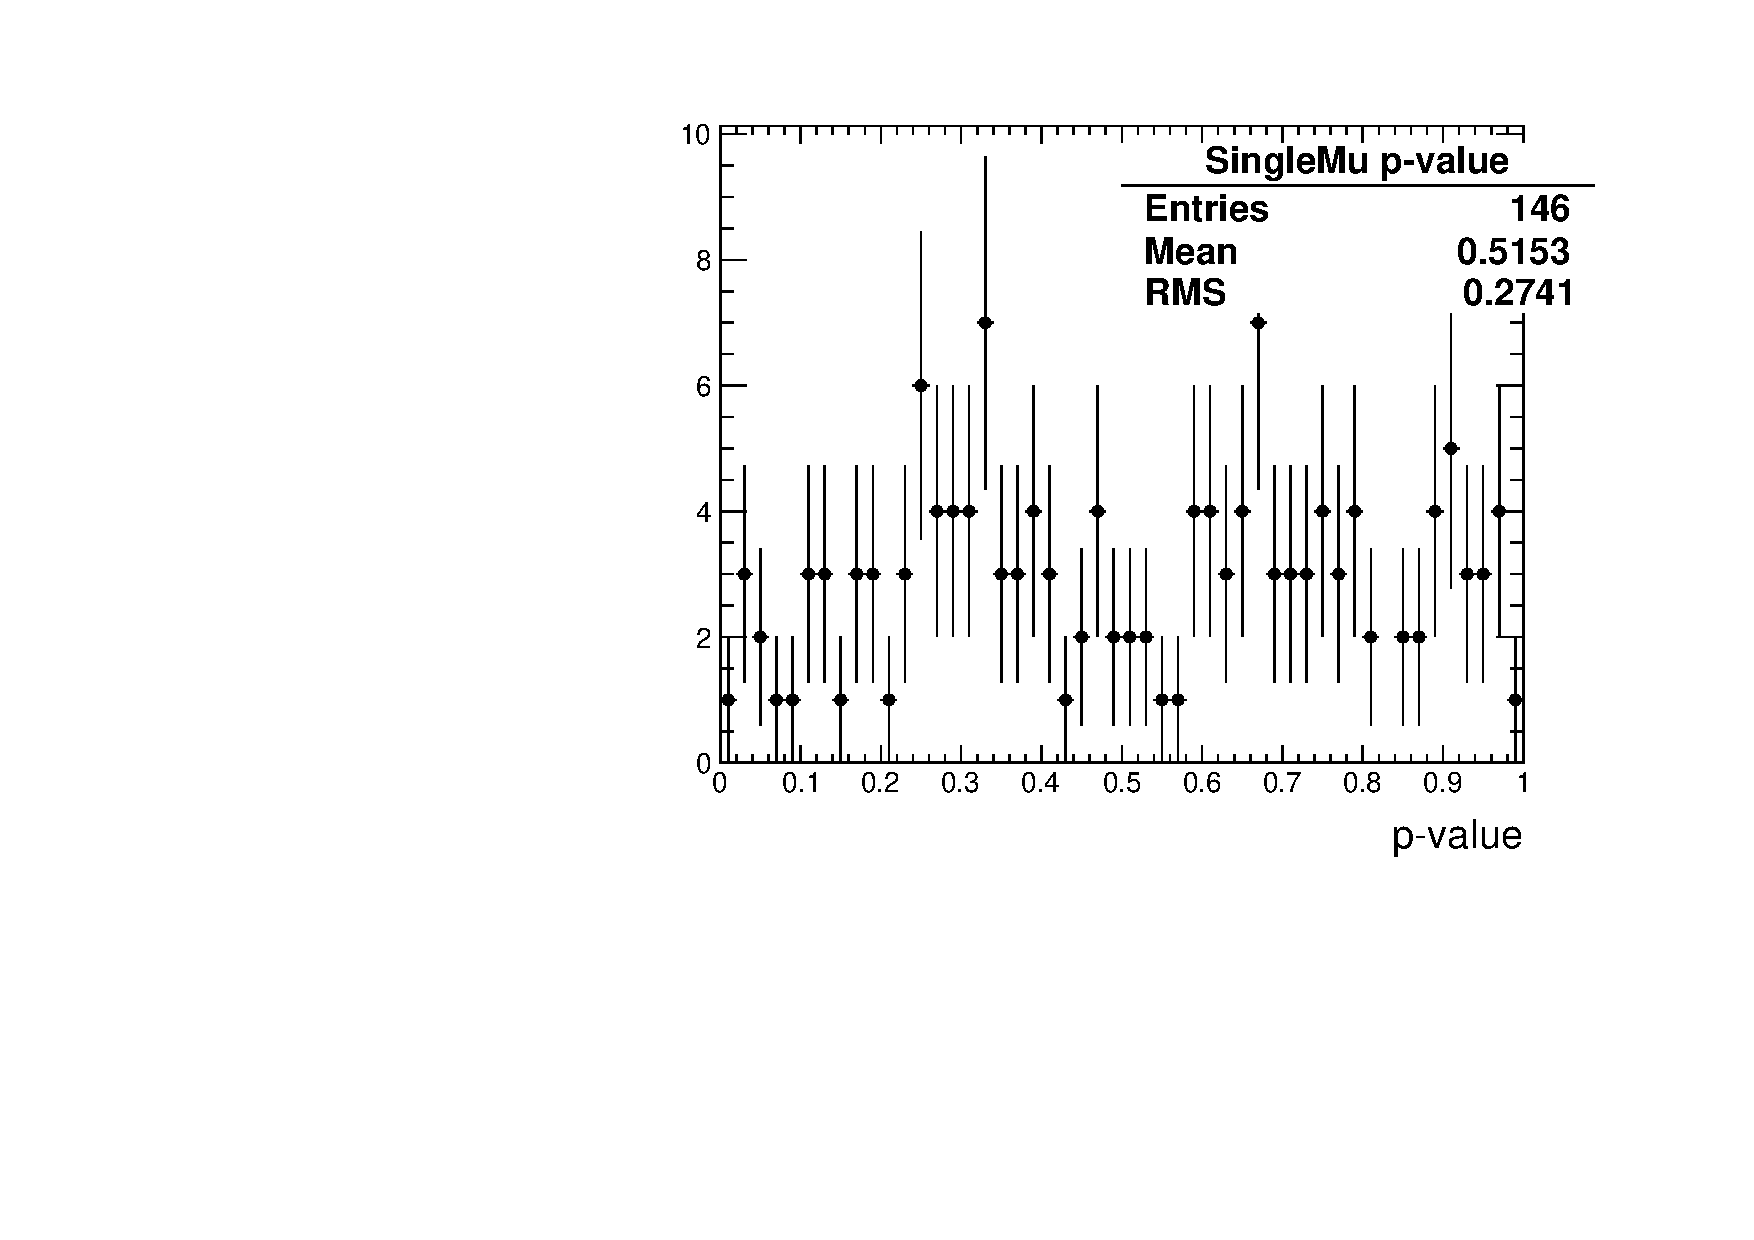
\includegraphics[width=0.5\textwidth]{figures/template2016Data/shapeOutputNewPU/scale_ht_variable_mht/SingleMu/fitOut/Linear2DShiftMean/pValue_Linear2DShiftMean_SingleMu.pdf}
  }~~
  \subfigure[\gj]{
    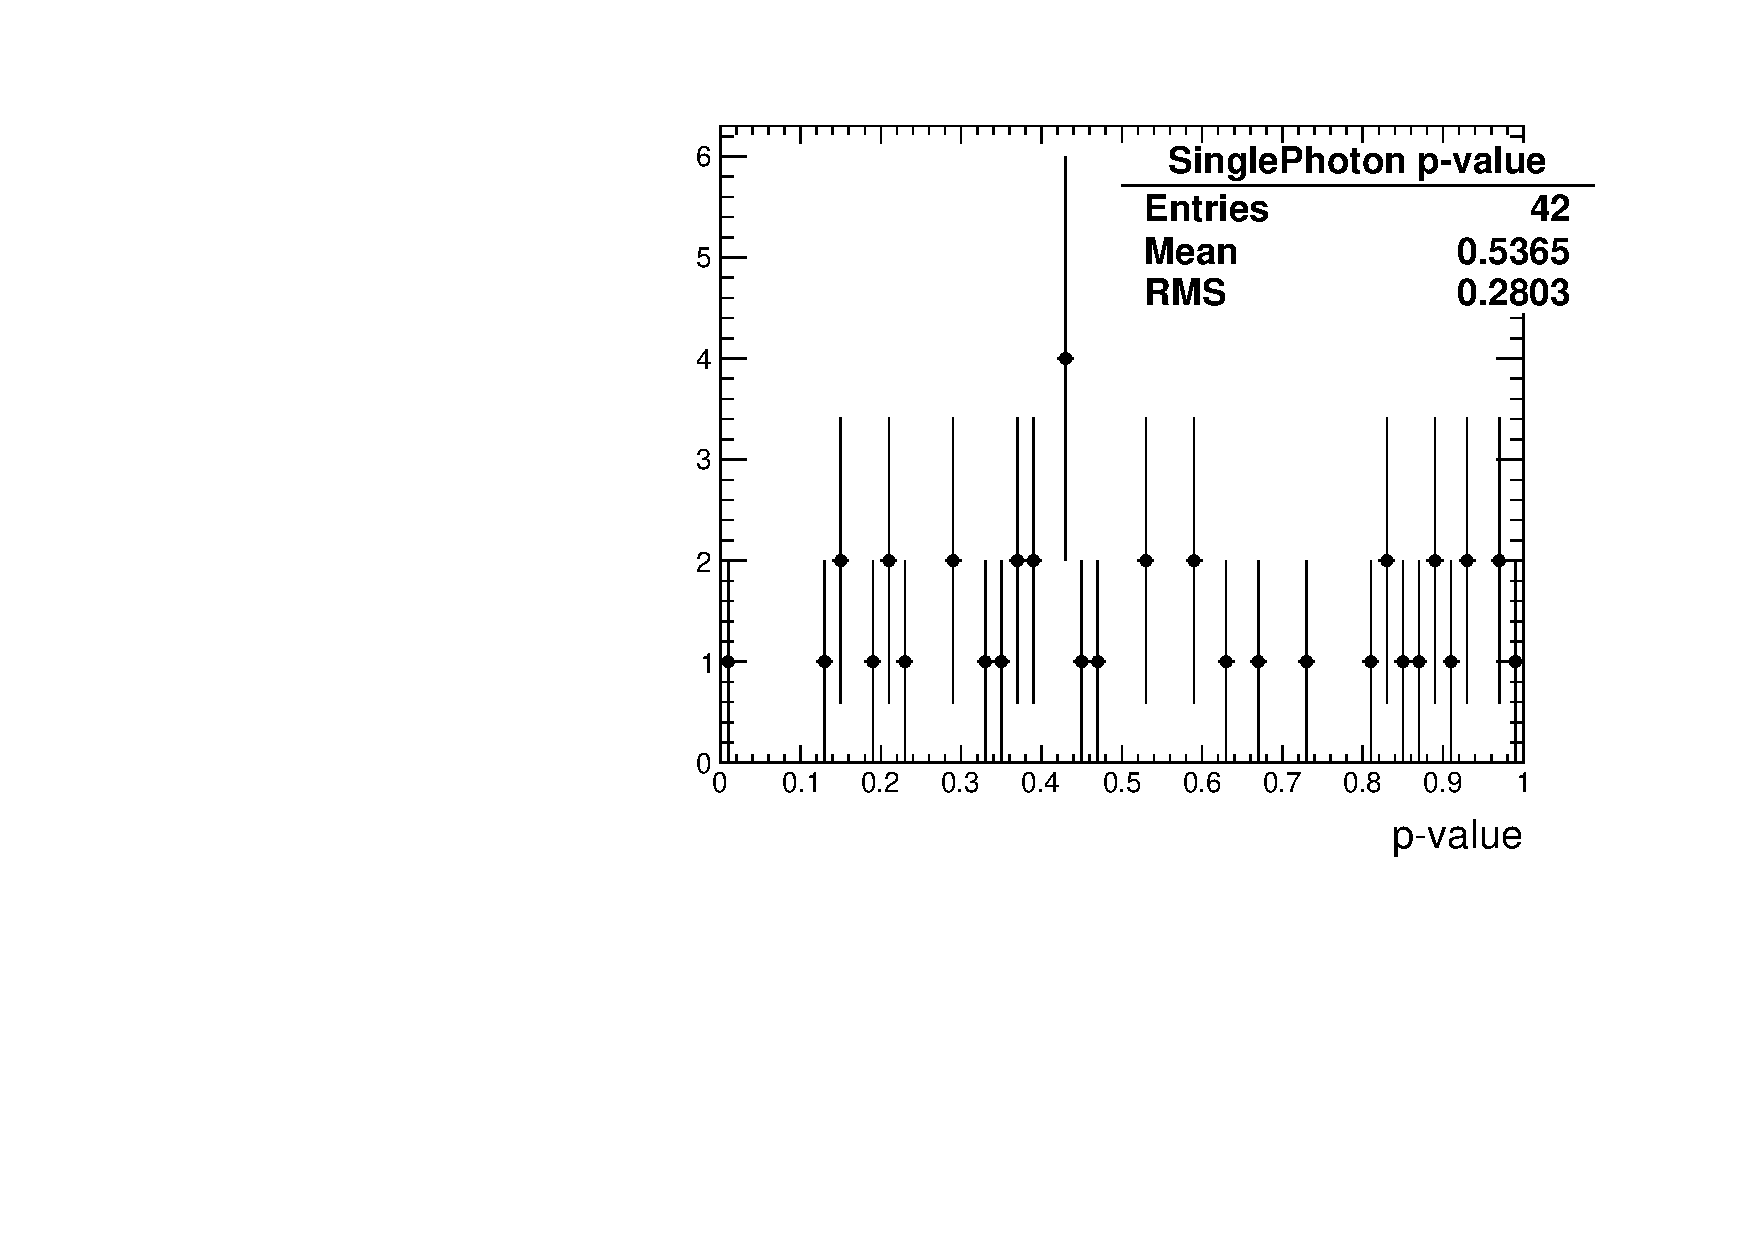
\includegraphics[width=0.5\textwidth]{figures/template2016Data/shapeOutputNewPU/scale_ht_variable_mht/SinglePhoton/fitOut/Linear2DShiftMean/pValue_Linear2DShiftMean_SinglePhoton.pdf}
  }\\
  \subfigure[\mmj]{
    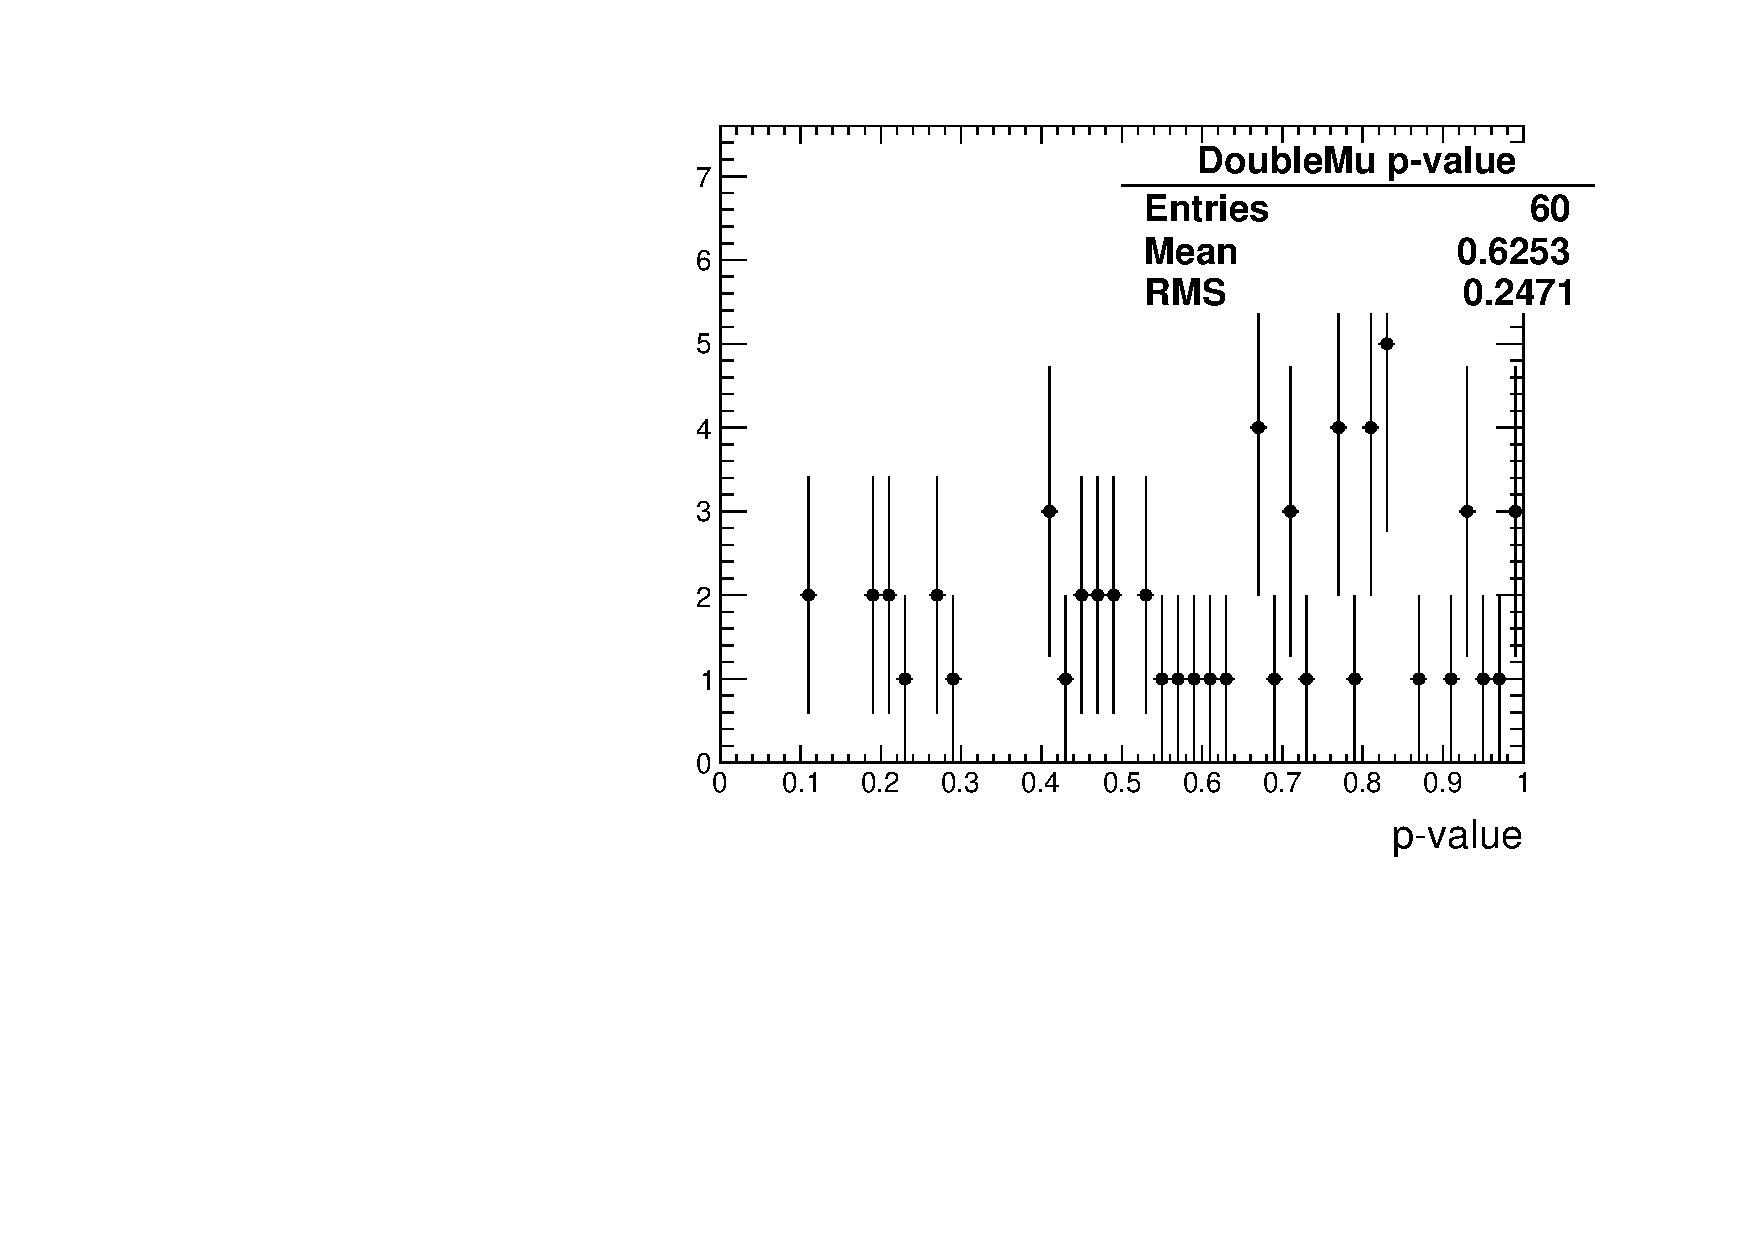
\includegraphics[width=0.5\textwidth]{figures/template2016Data/shapeOutputNewPU/scale_ht_variable_mht/DoubleMu/fitOut/Linear2DShiftMean/pValue_Linear2DShiftMean_DoubleMu.pdf}
  }~~
  \\
  \caption{\label{fig:pValues} The distributions of the p-value for the linear fit.} 
\end{figure}
\subsection{Deriving systematics on the \texorpdfstring{\mht}~dimension}
\label{sec:systMhtDimension}
The systematic in the \mht dimension is extracted from the hypothesis
of no bias. This is done by using the control regions 
to determine the statistical precision to which this hypothesis can
be confirmed. This information is then used to derive the systematic 
uncertainty, as described in the following. 

Each background in the signal region (\ttbar/W  and \zInv~) is predicted 
using several control regions. In order to determine the uncertainty in
the \mht dimension a combined linear fit is made over all relevant control regions
of the linear function. A requirement of at least 10 events and a non-trivial
number of degrees of freedom is made to ensure a reasonable fit. Where this
requirement is not satisfied the \mht distribution is not used in the signal region.
An \mht requirement of 130 \GeV is made to ensure a similar phase space to 
the signal region (this maps the minimum \mht due to the \alt requirements in the signal region).
The uncertainty on the linear parameter from the fit is then
used to define the up and down one sigma variations of the nominal template.
As a conservative estimate, the best fit value of the parameter is 
added in quadrature to its uncertainty in order to derive the overall variation.

Example templates with this uncertainty are shown in Fig.~\ref{fig:mht-templates}
in Sec.~\ref{sec:results}. Here the template variations for both relevant 
backgrounds are combined to show the overall uncertainty on the \mht dimension. 
The scatter of the points around one is compatible with statistical fluctuations.

An additional validation is carried out by comparing expected and observed uncertainties
on the linear parameter defining the template variations.
The expected uncertainties are derived by using a linear fit to the MC/MC ratio where the numerator
have uncertainties given by the Poisson uncertainty on the number of predicted counts while
the uncertainty on the denominator comes from the statistical uncertainty on the
MC prediction. The relative uncertainties per 100 \GeV from the weighted mean of \mht
for \ttbar/W and \zInv~ are shown in Fig.~\ref{fig:expectedObservedTtw} 
and Fig.~\ref{fig:expectedObservedZinv} and compared to those observed.
These show good agreement which provides additional motivation for the 
zero bias hypothesis as well as validating the method for deriving expected uncertainties.
%%%ADD WHEN UNLIND!!
% As an additional gauge of the effect of the template variations the uncertainty parameter 
% can be translate to an uncertainty on the last bin. This is typically
% of the order of 10-100\% depending on the category and is shown
% in Fig.~\ref{fig:frenchFlagLastBin}.


\begin{figure}[h!]
  \centering
  \subfigure[\label{fig:expectedTtw} Expected uncertainties]{
    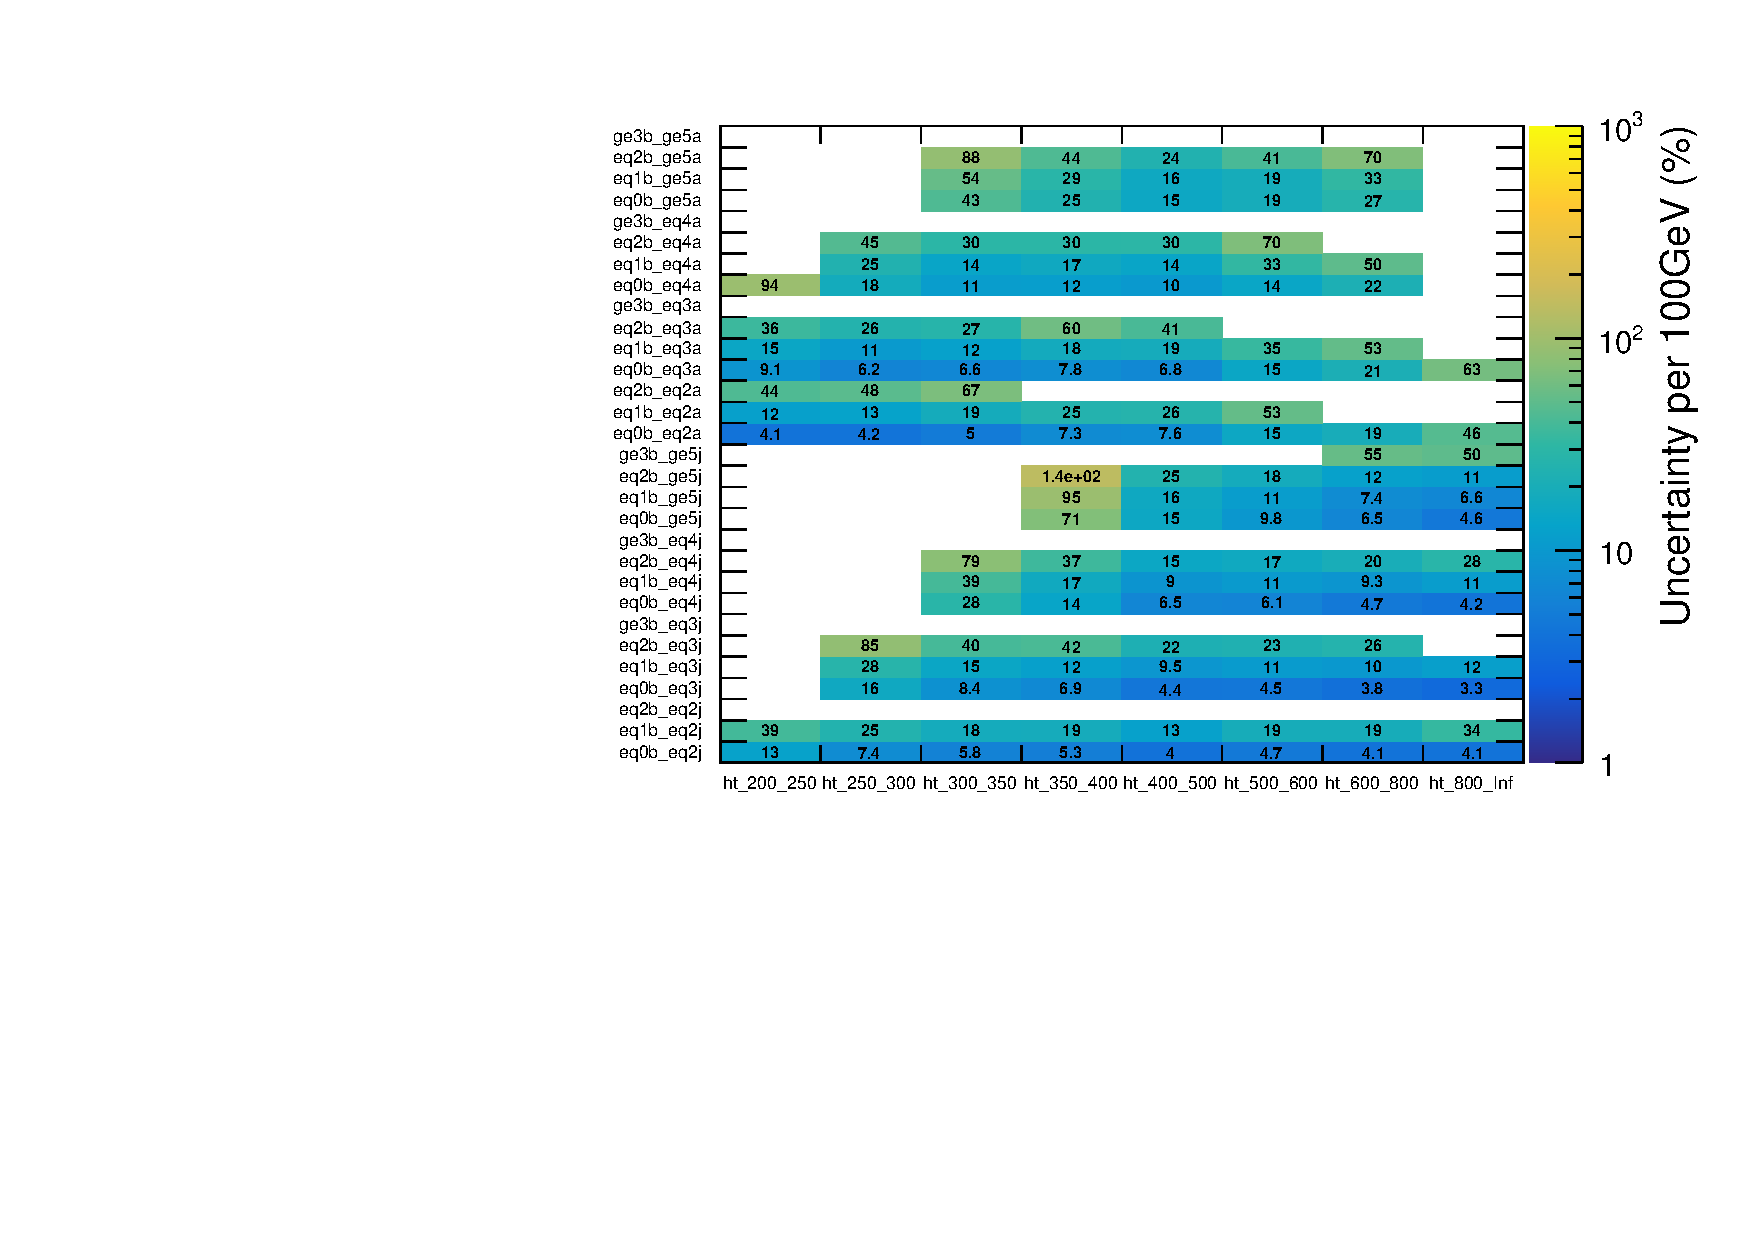
\includegraphics[width=0.5\textwidth]{figures/template2016Data/shapeOutputNewPUMC/scale_ht_variable_mht/Ttw/fitOut/Linear2DShiftMean/frenchFlagErrComplete_Linear2DShiftMean_p1_Ttw.pdf}
  }~~
  \subfigure[\label{fig:observedTtw} Observed uncertainties]{
    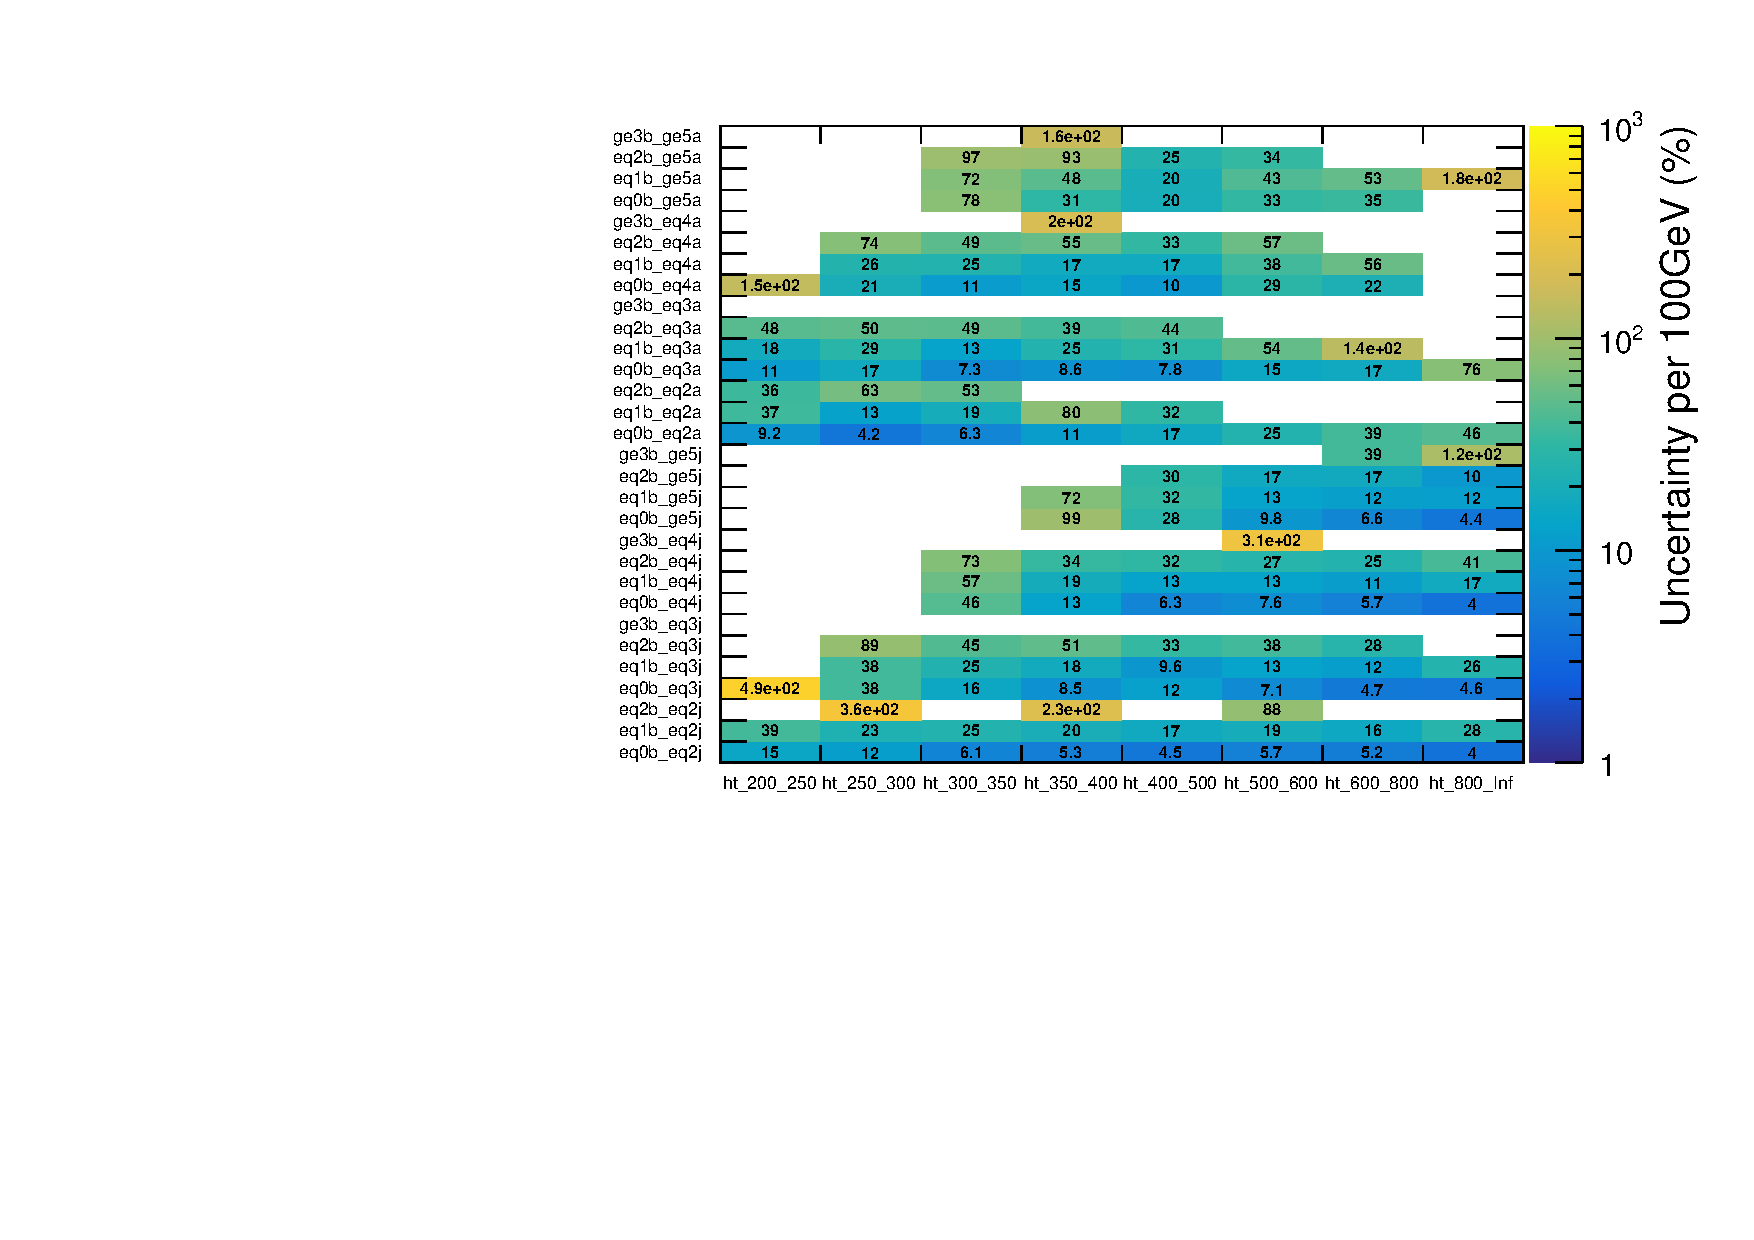
\includegraphics[width=0.5\textwidth]{figures/template2016Data/shapeOutputNewPU/scale_ht_variable_mht/Ttw/fitOut/Linear2DShiftMean/frenchFlagErrComplete_Linear2DShiftMean_p1_Ttw.pdf}
  }\\
  \caption{\label{fig:expectedObservedTtw} Expected relative uncertainties per 100 \GeV shown for \ttbar/W in Fig.~\ref{fig:expectedTtw} are consistent
  with observed uncertainties shown in Fig.~\ref{fig:observedTtw}.}
\end{figure}

\begin{figure}[h!]
  \centering
  \subfigure[\label{fig:expectedZinv} Expected uncertainties]{
    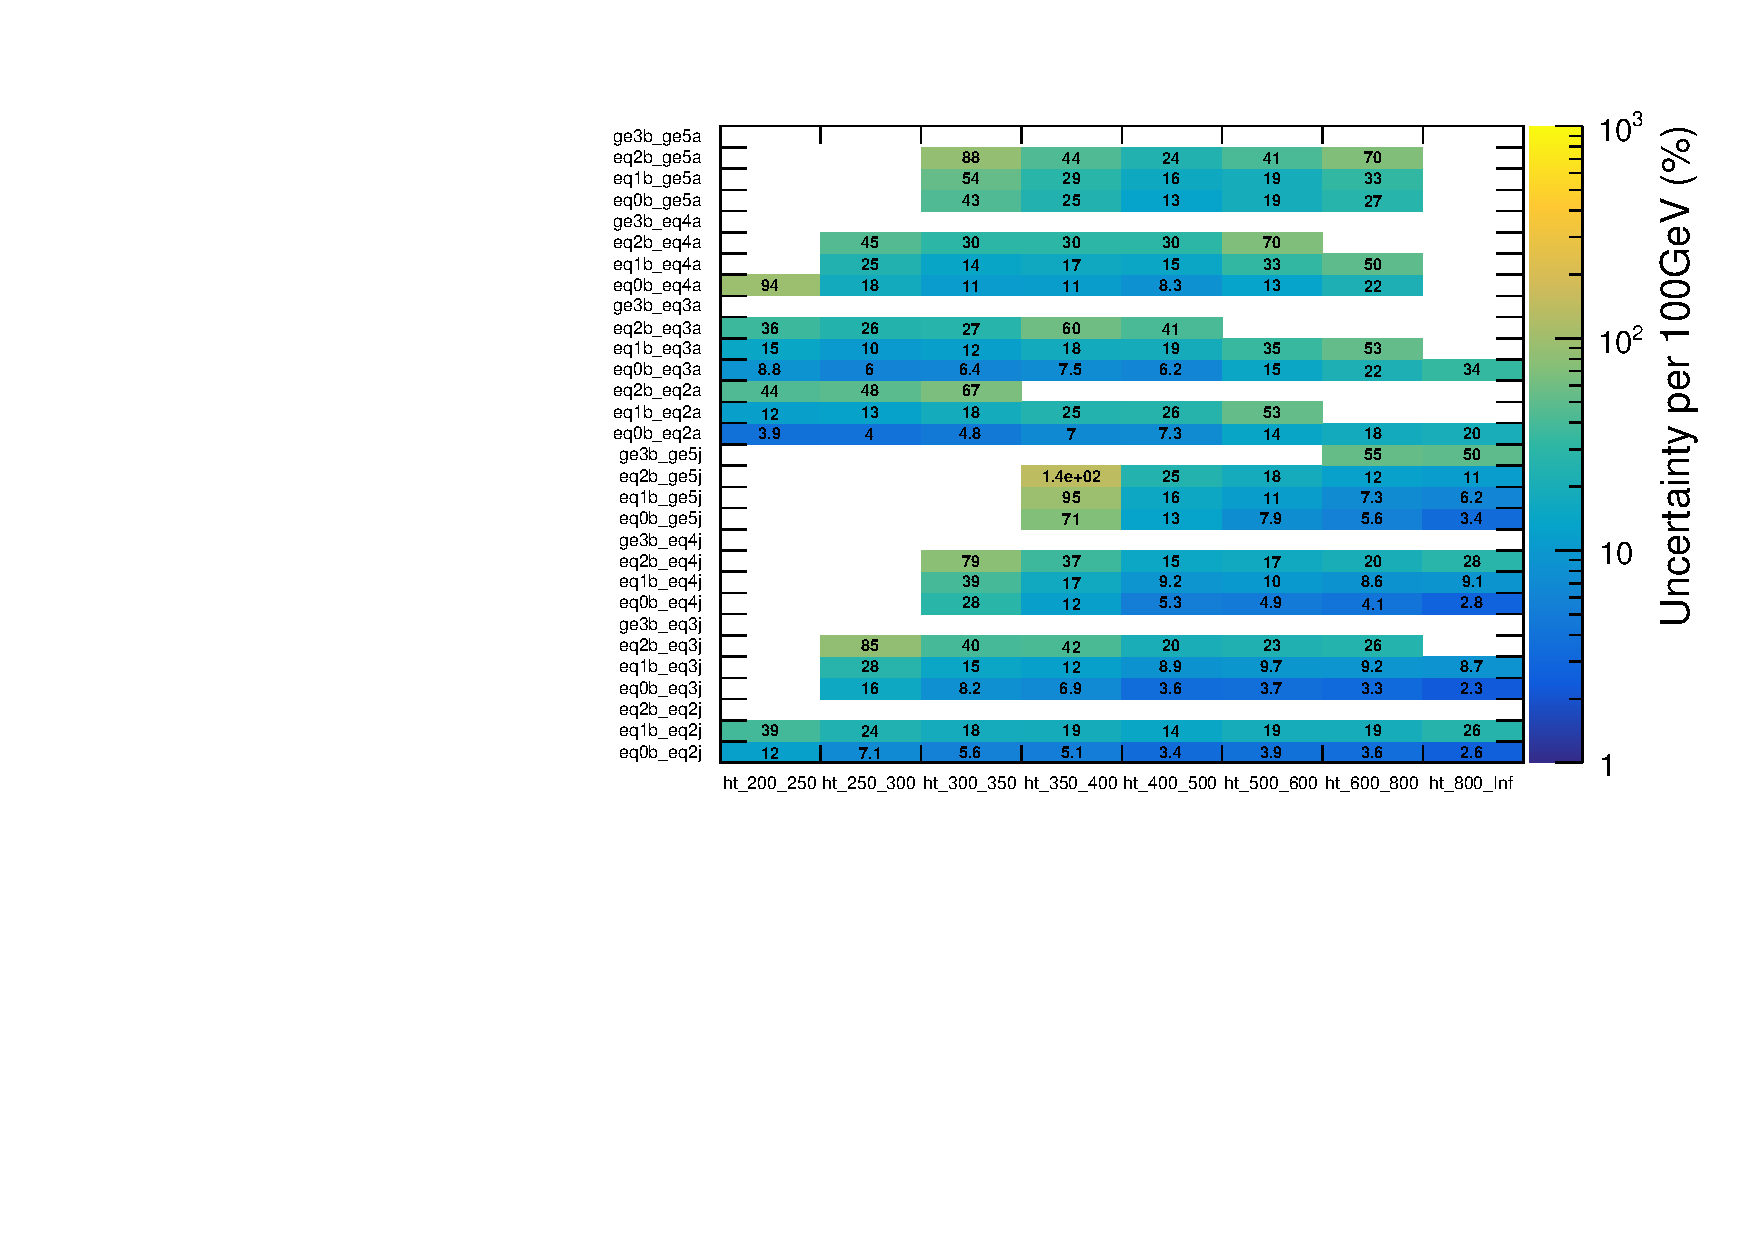
\includegraphics[width=0.5\textwidth]{figures/template2016Data/shapeOutputNewPUMC/scale_ht_variable_mht/Zinv/fitOut/Linear2DShiftMean/frenchFlagErrComplete_Linear2DShiftMean_p1_Zinv.pdf}
  }~~
  \subfigure[\label{fig:observedZinv} Observed uncertainties]{
    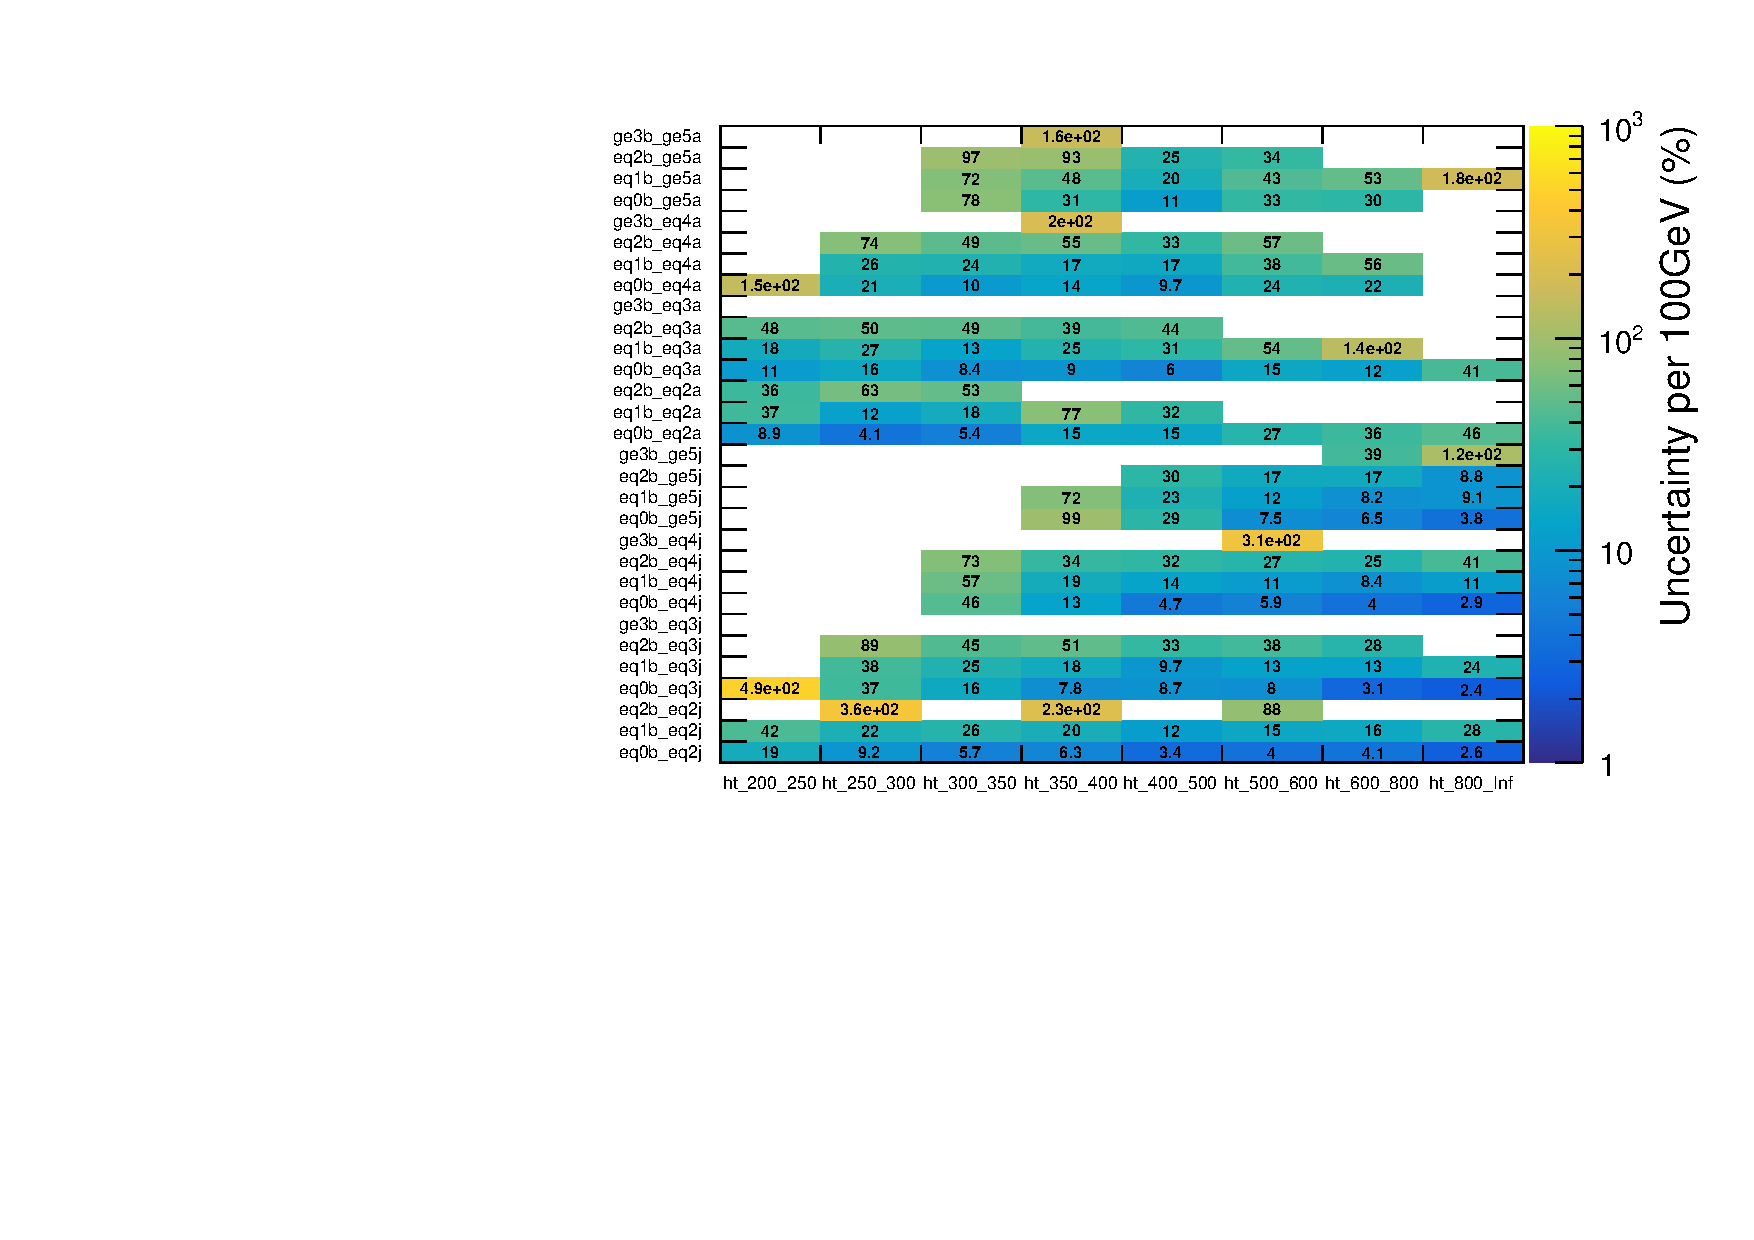
\includegraphics[width=0.5\textwidth]{figures/template2016Data/shapeOutputNewPU/scale_ht_variable_mht/Zinv/fitOut/Linear2DShiftMean/frenchFlagErrComplete_Linear2DShiftMean_p1_Zinv.pdf}
  }\\
  \caption{\label{fig:expectedObservedZinv}Expected relative uncertainties per 100 \GeV shown for \zInv~ in Fig.~\ref{fig:expectedZinv} are consistent
  with observed uncertainties shown in Fig.~\ref{fig:observedZinv}.}
\end{figure}


% \begin{figure}[h!]
%   \centering
%   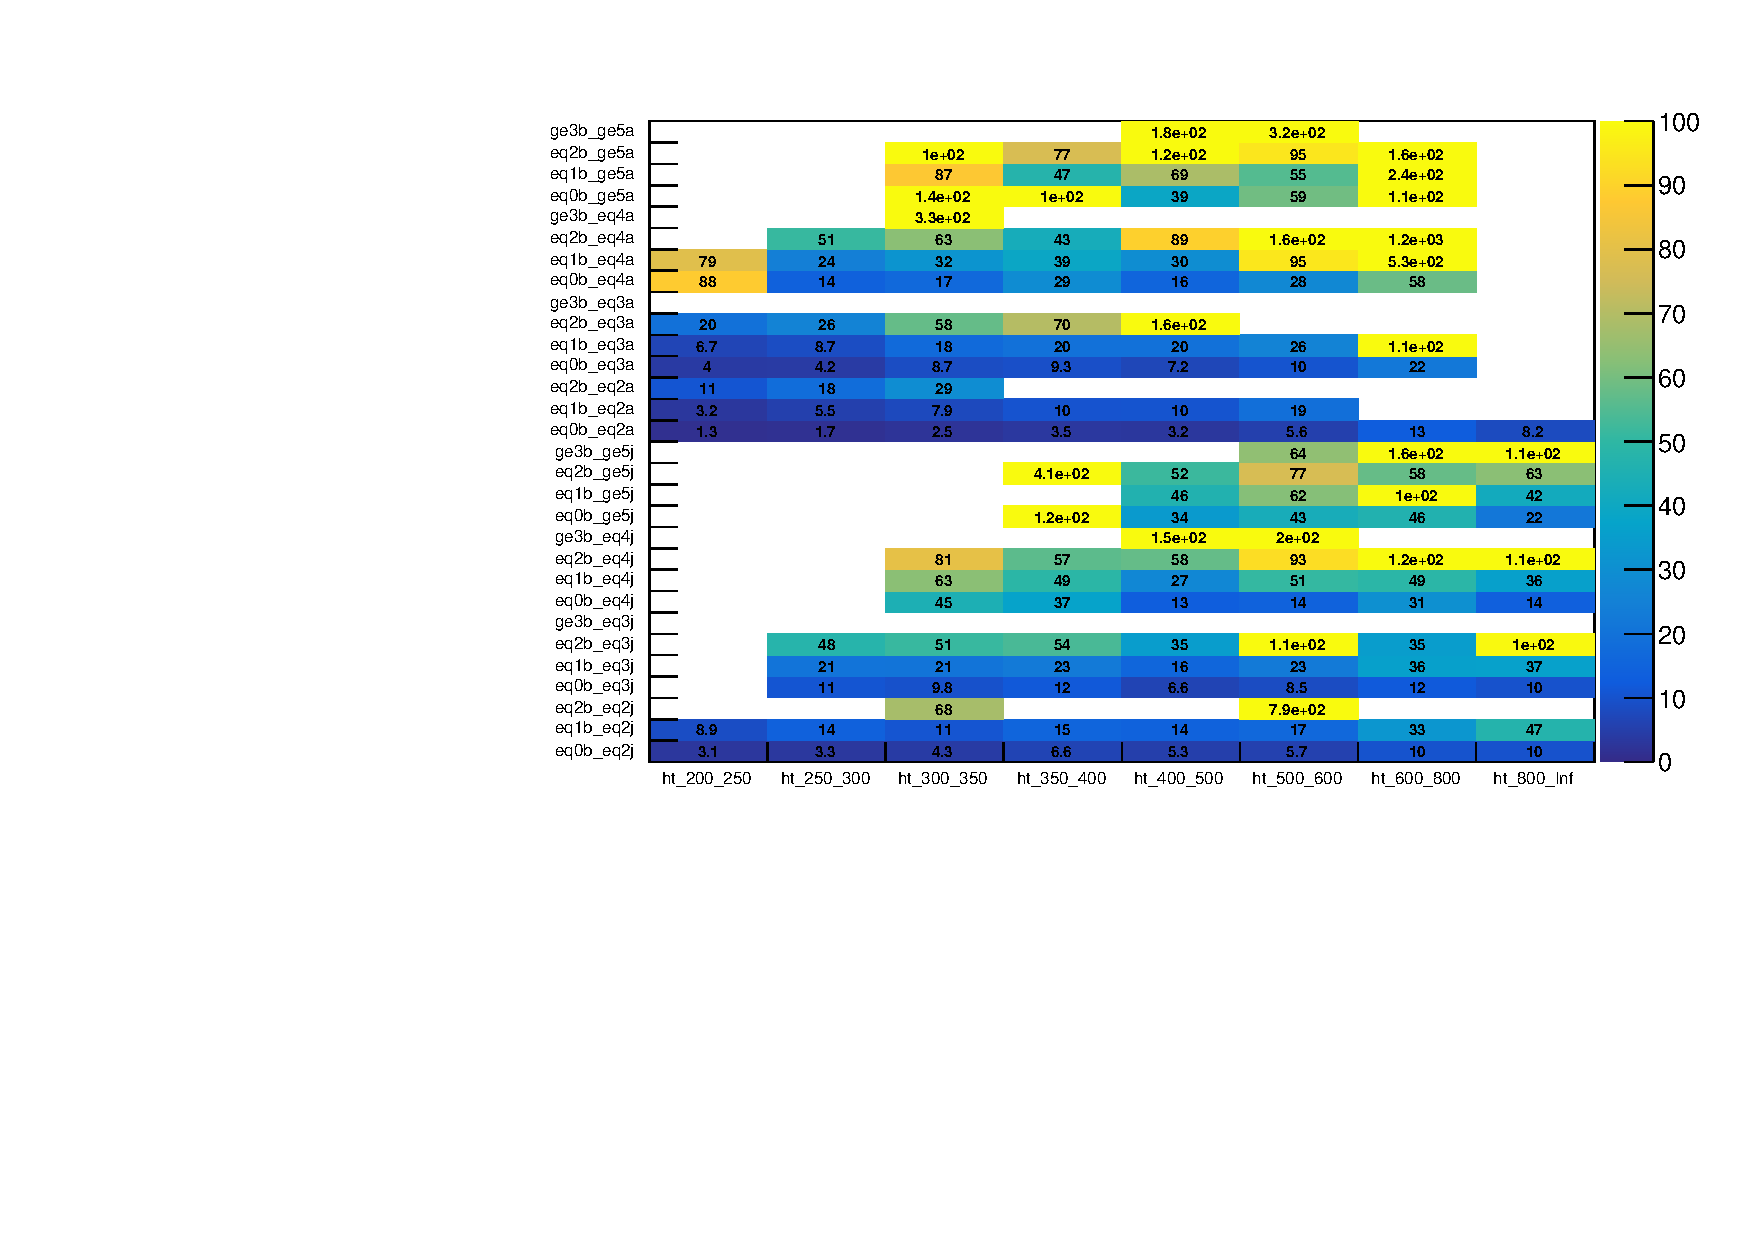
\includegraphics[width=0.8\textwidth]{figures/template13TeV/2p2fb/frenchFlagLastBin.pdf}
%   \caption{\label{fig:frenchFlagLastBin} Observed uncertainties in the 
%   last bin of \mht over all categories and \scalht bins for 2.2\ifb.}
% \end{figure}

\newpage
\subsection{Comparison to known systematic sources}
\label{sec:mcSystStudiesShape}
To further validate the data driven procedure a range of known systematic sources are studied.
The size of the variation of the \mht distribution under $\pm1\sigma$ shifts of these sources is compared 
to that of the orthogonal polynomial systematic described in \ref{sec:valid13} to ensure they are
covered. The sources considered are the b-tag scale factor uncertainty, jet energy correction uncertainty, 
pile-up reweighting uncertainty, and top \Pt rewieghting uncertainty. For each source of systematic the prediction
is varied by $\pm1\sigma$. To study the effect of this systematic variation on the \mht dimension, and not normalisation, 
the resulting template is normalised to the nominal template in each jet category and \scalht bin. 
These systematic effects can then be compared to the data-driven orthogonal polynomial systematic. 

Figures~\ref{fig:mcCompLow} and \ref{fig:mcCompHigh} show the representative exampltes for two different \scalht 
bins and jet-categories. As can be seen in each case the \mht dimension change under the variation of all 
systematics considered is easily contained within the orthogonal polynomial variation. 
To show the effect across all jet categories, except the monojet categories for which the \mht dimension is not used,
and \scalht bins Fig~\ref{fig:lastBinVar} shows the maximum upwards/downwards variation in the last 
\mht bin as a proportion of the orthogonal polynomial variation. In almost all bins this is shown to be 
significantly less than unity confirming that the orthogonal polynomial can cover the known systematic
deviations.

\begin{figure}[h!]
  \centering
  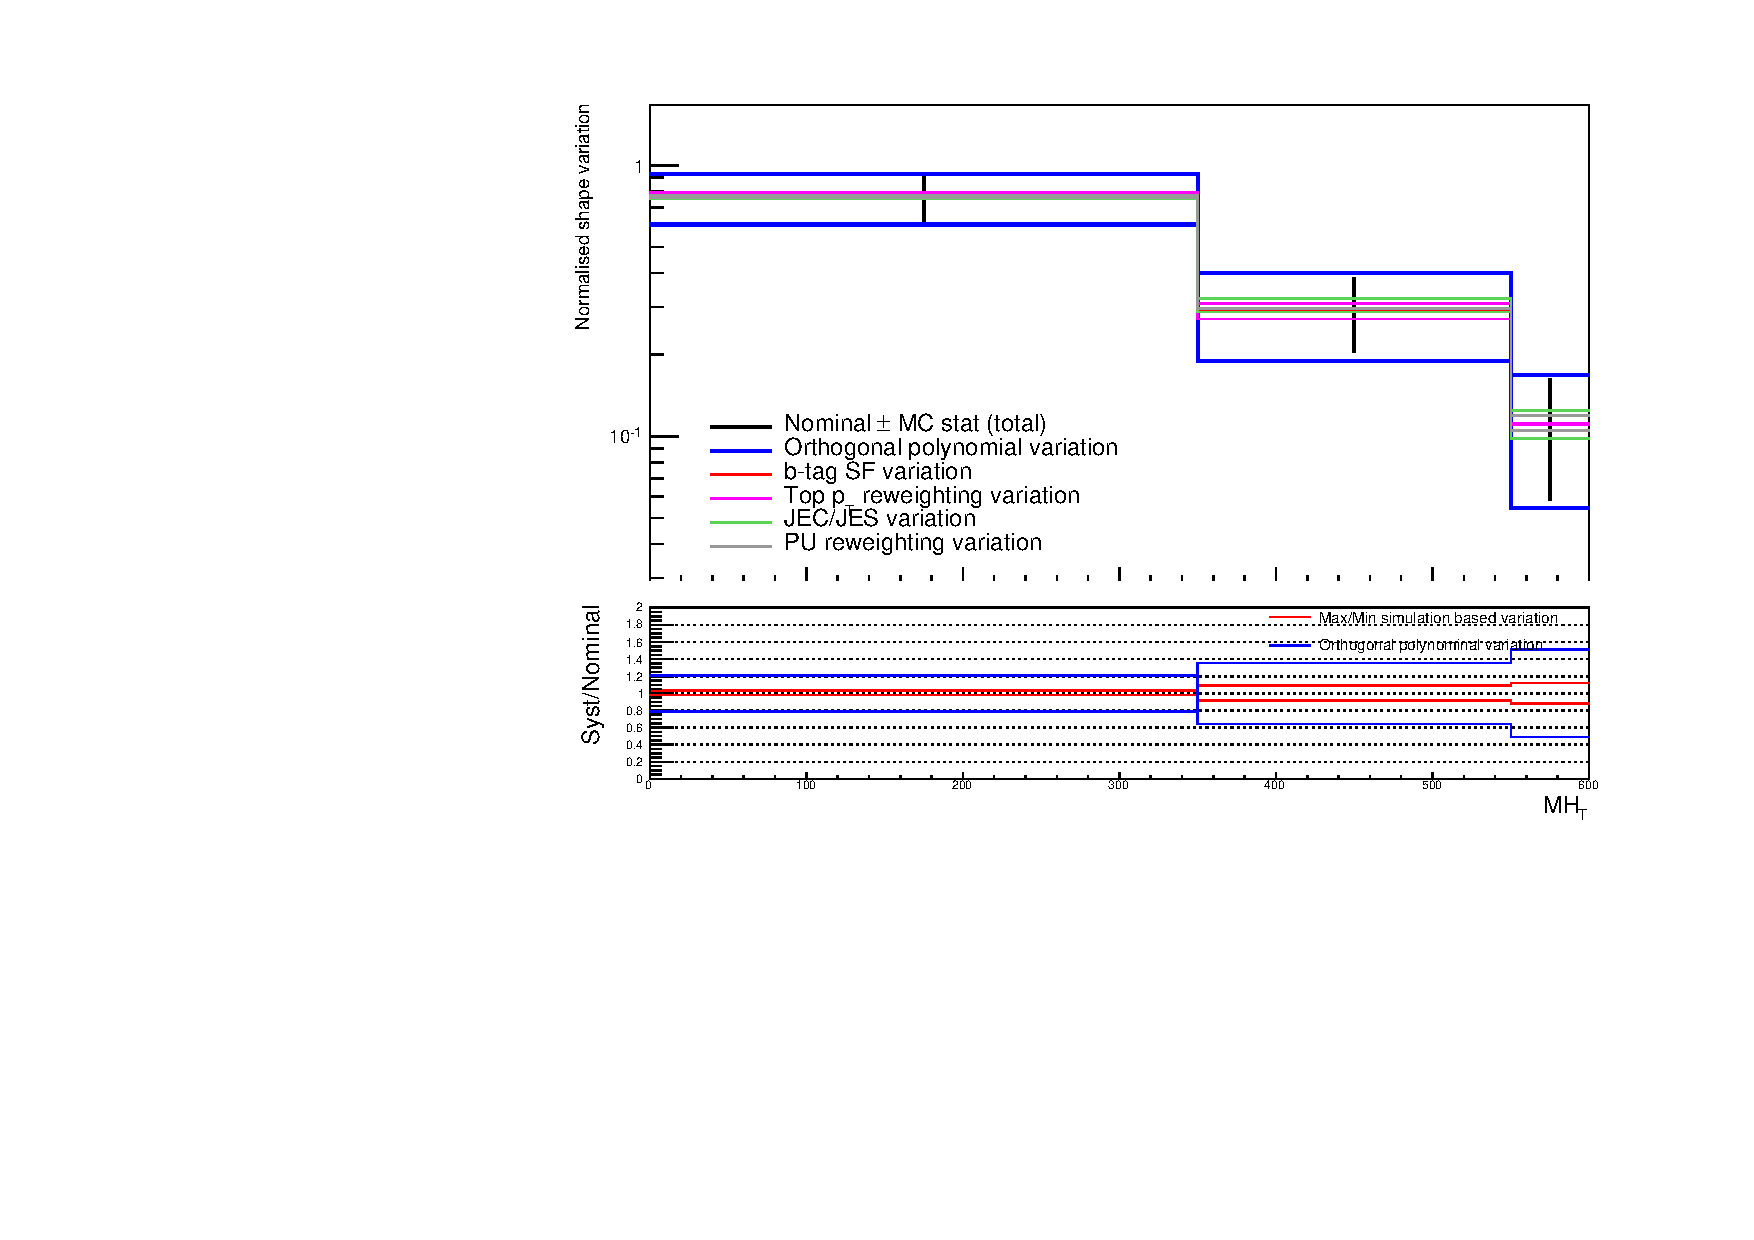
\includegraphics[width=0.8\textwidth]{figures/template13TeV/mcComparison/totalSMS-T1bbbb_mGluino-1400_mLSP-800_25ns_mht_ge5j_ge3b_800.pdf} 
  \caption{\label{fig:mcCompLow} MC based systematic variations shown to be considerably smaller 
  than the orthogonal polynomial data-driven systematic for an example bin \scalht $800-\infty$, \njet $\geq 5$, \nb $\geq 2$.}
\end{figure}
\begin{figure}[h!]
  \centering
  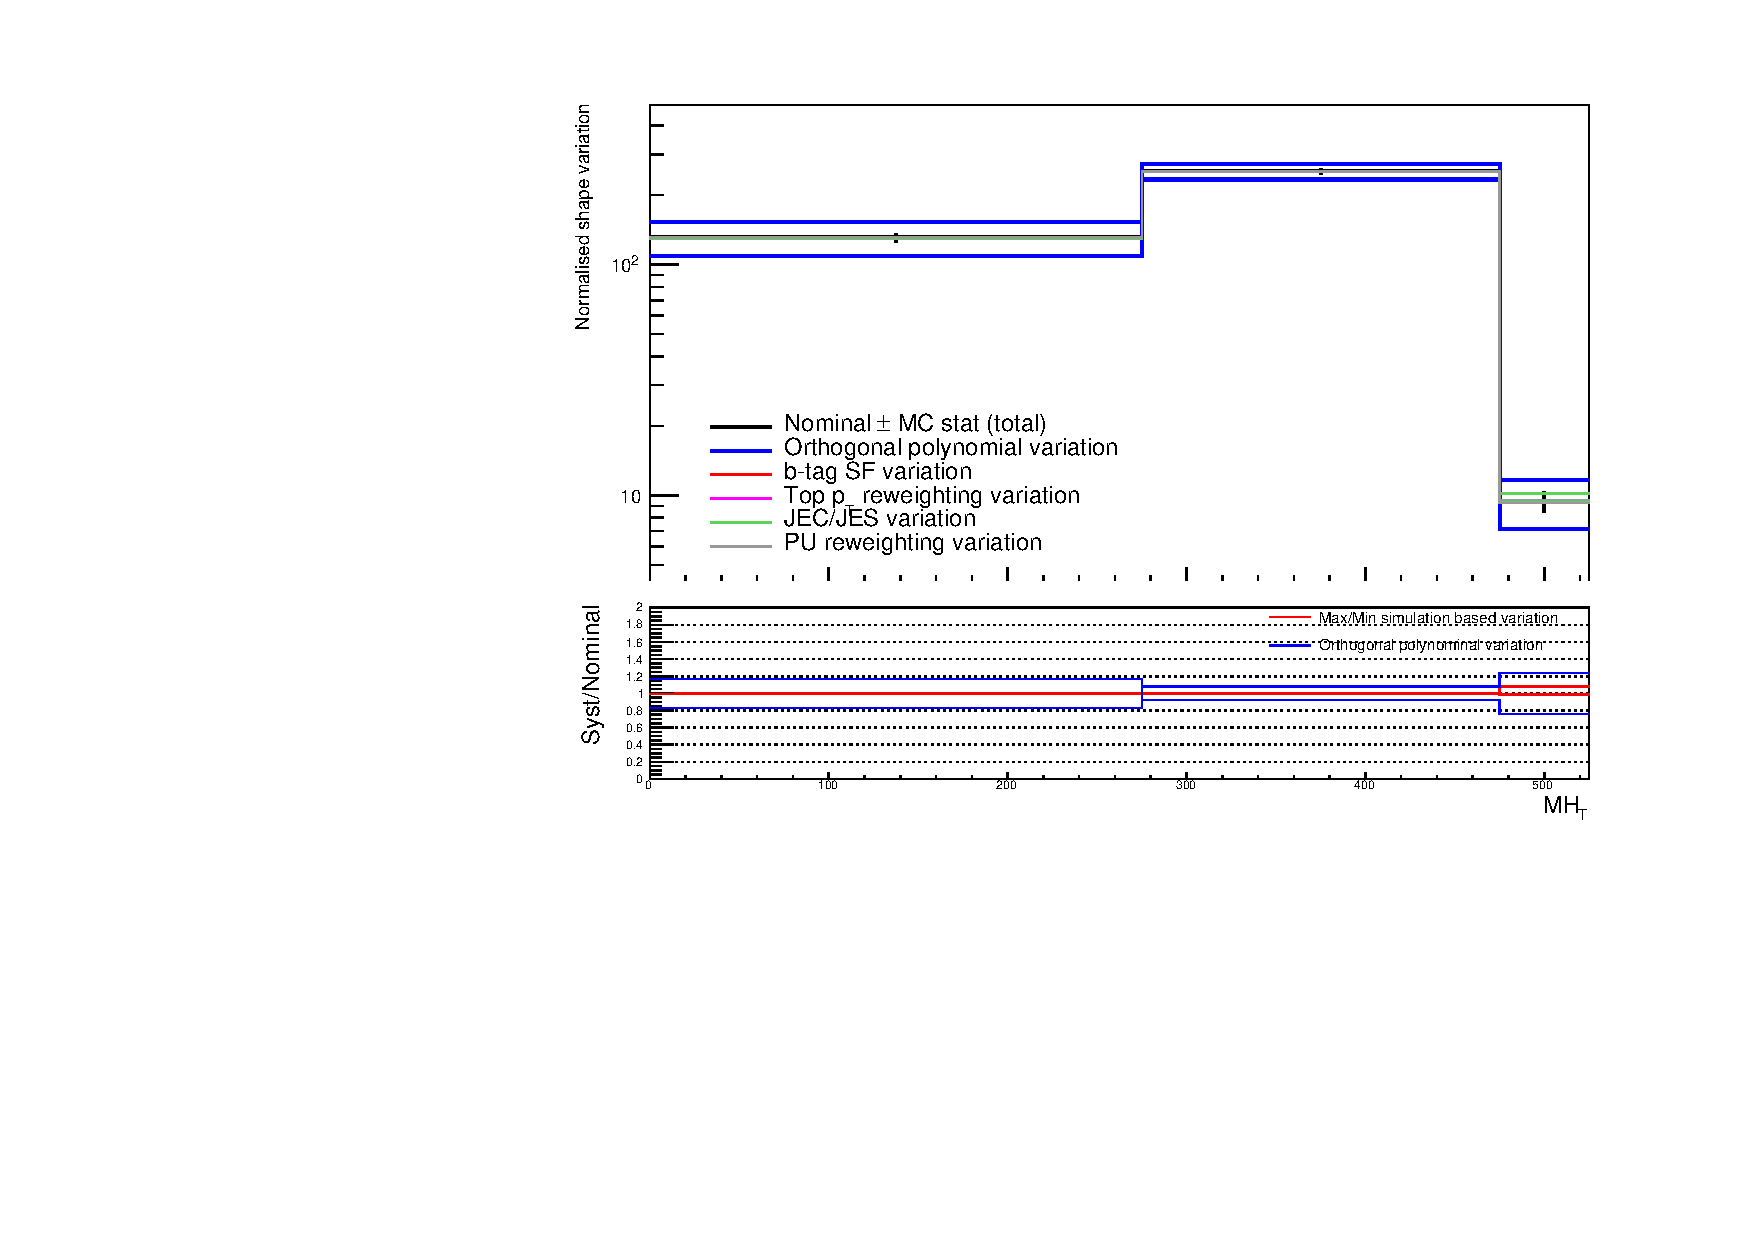
\includegraphics[width=0.8\textwidth]{figures/template13TeV/mcComparison/totalSMS-T1bbbb_mGluino-1400_mLSP-800_25ns_mht_eq2j_eq0b_400.pdf} 
  \caption{\label{fig:mcCompHigh} MC based systematic variations shown to be considerably smaller 
  than the orthogonal polynomial data-driven systematic for an example bin \scalht 400-500, \njet $= 2$, \nb $= 0$.}
\end{figure}

\begin{figure}[h!]
\centering
\subfigure[Upwards deviation]{
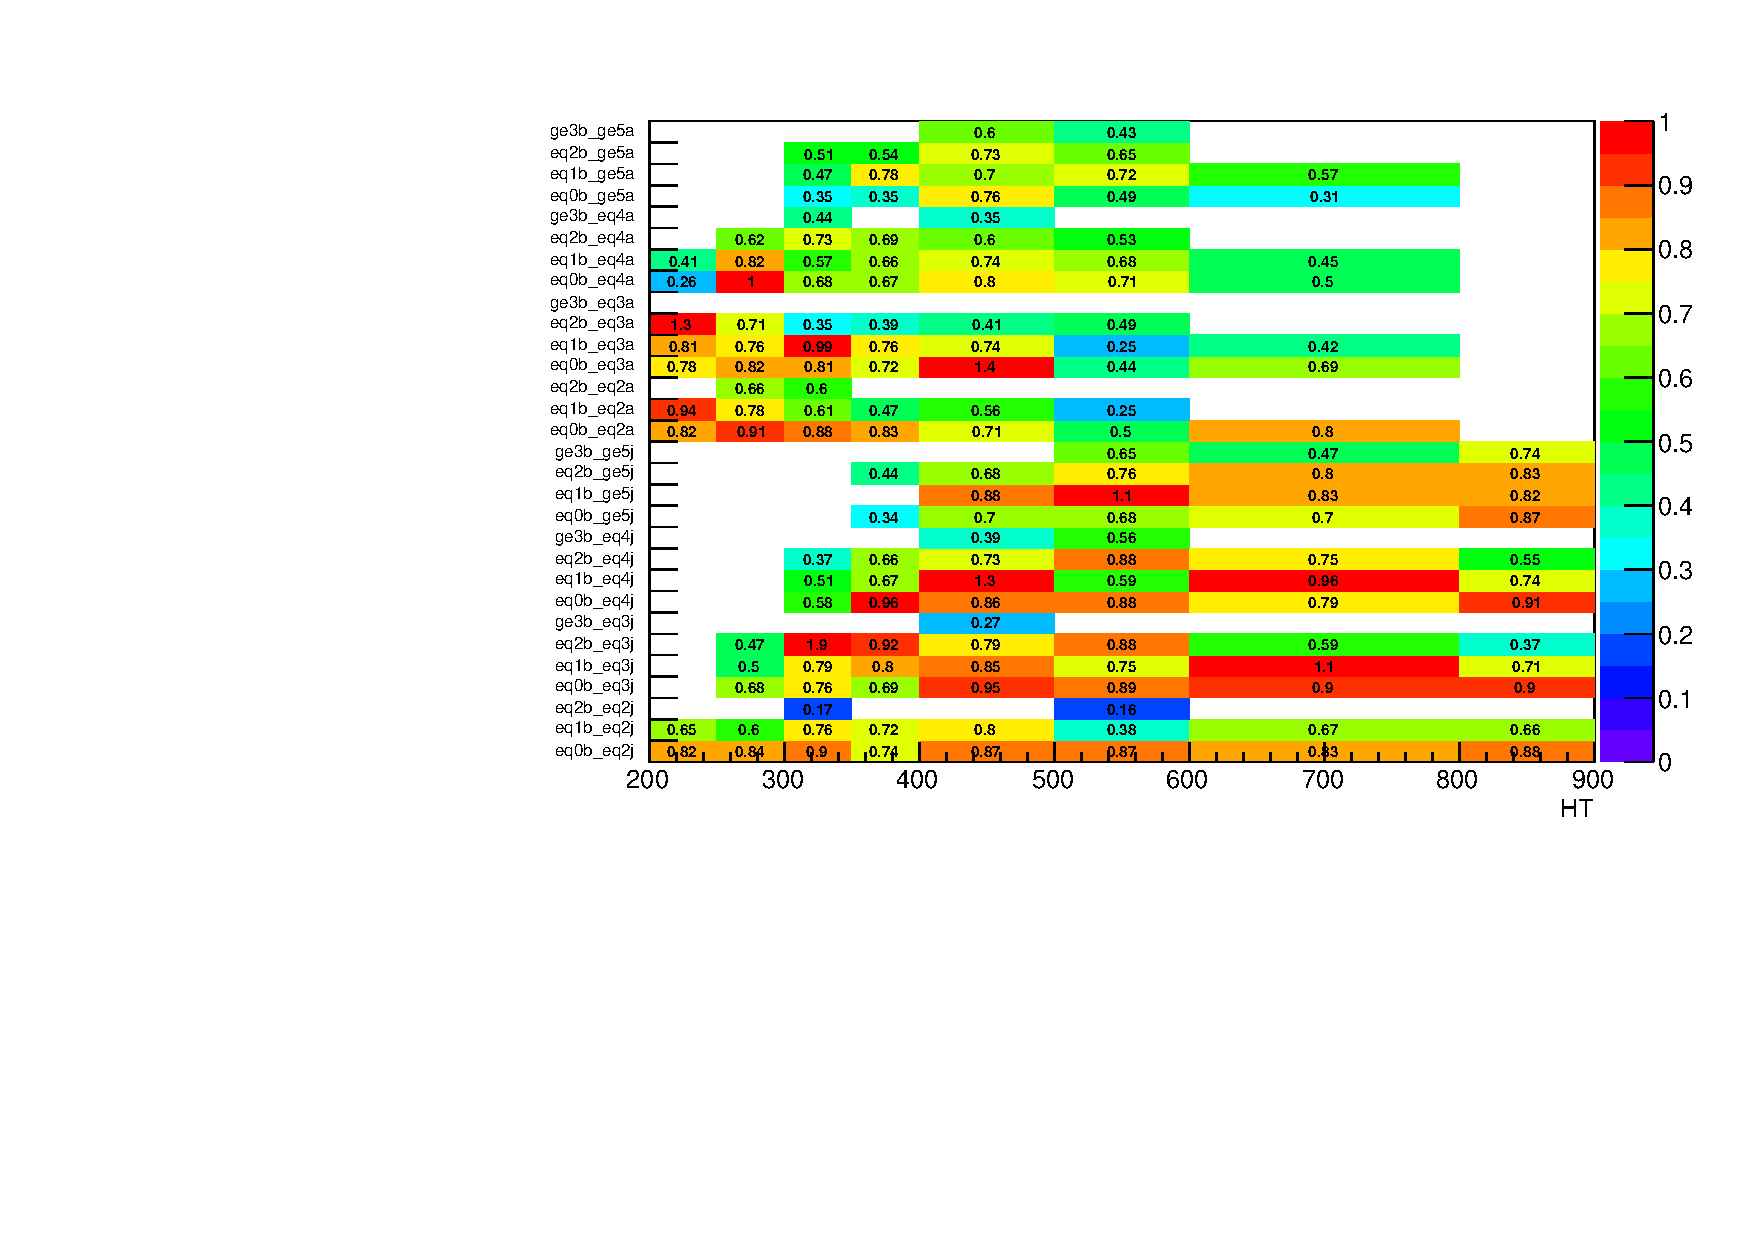
\includegraphics[width=0.5\textwidth]{figures/template13TeV/mcComparison/lastBinRatioMax.pdf}
}
\subfigure[Downwards deviation]{
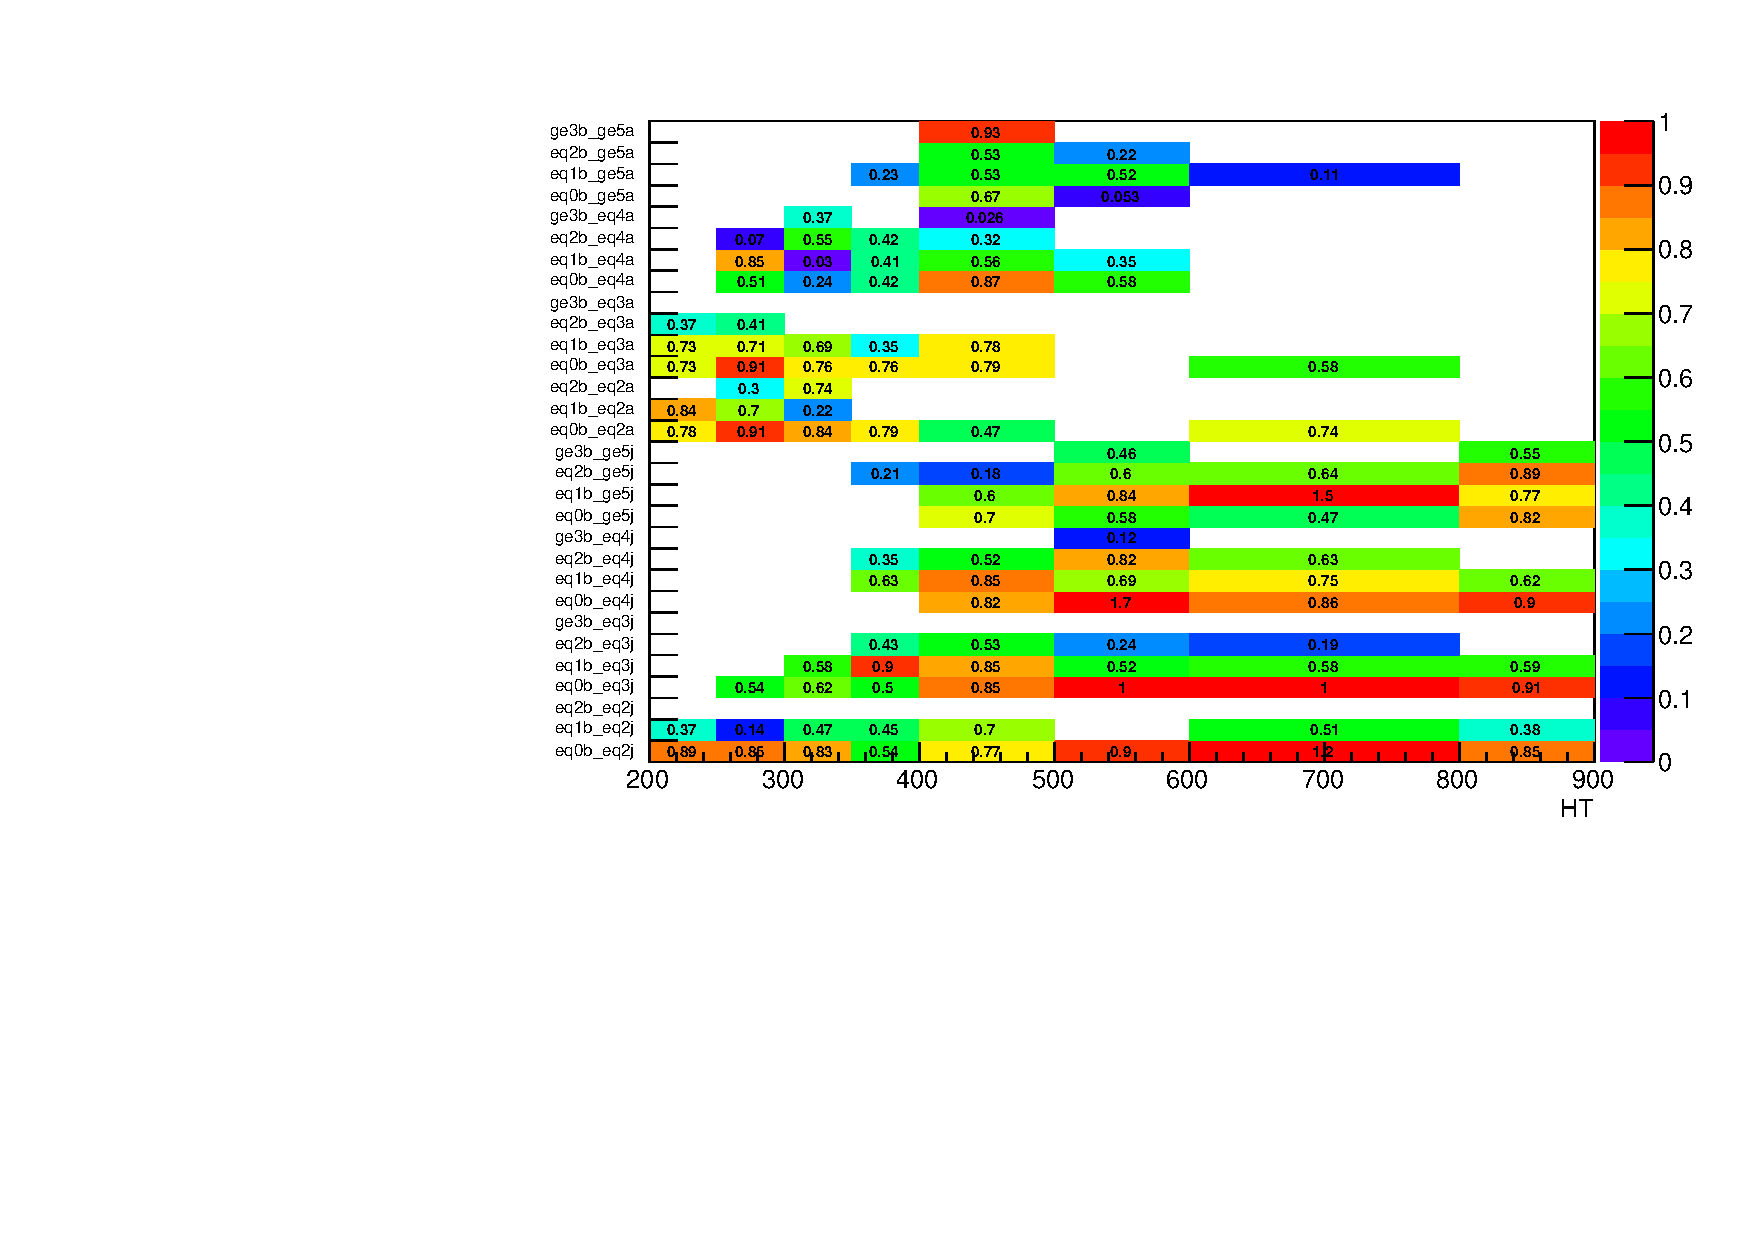
\includegraphics[width=0.5\textwidth]{figures/template13TeV/mcComparison/lastBinRatioMin.pdf}
}\\
\caption{\label{fig:lastBinVar} Maximum upwards and downwards variations in the last \mht bin as a proportion of the orthogonal polynomial deviation}
\end{figure}
